\documentclass[a4paper,10pt]{article}

\usepackage[T1]{fontenc}
\usepackage[utf8]{inputenc}

\usepackage{amsmath}
\usepackage{amssymb}

\usepackage{xcolor}
\usepackage{graphicx}
\usepackage{grffile}

\usepackage{subcaption}

\usepackage{booktabs}

\title{Bayesian Sparsification of $\cplx$-valued networks}
\author{Ivan Nazarov, and Evgeny Burnaev}

%% notation
\newcommand{\real}{\mathbb{R}}
\newcommand{\cplx}{\mathbb{C}}
\newcommand{\tr}[1]{\mathop{tr}{#1}}

\newcommand{\hop}{{\mkern-1.5mu\dagger}}
\newcommand{\conj}[1]{\overline{#1}}

% \renewcommand{\top}{{\mkern-1.5mu\intercal}}
\renewcommand{\vec}[1]{\overrightarrow{#1}}
\newcommand{\diag}[1]{\mathrm{diag}{#1}}

%% drafting macro
\newcommand{\important}[1]{\textbf{\color{red} #1}}
\newcommand{\attn}[2]{\textbf{\color{red} #2~\textsuperscript{\textit{[#1]}}}}
\newcommand{\verify}[1]{\attn{verify}{#1}}
\newcommand{\rewrite}[1]{\attn{rewrite}{#1}}
\newcommand{\todo}[1]{{\color{blue} [TODO]} \important{#1}}

%% red-highlight missing citations
\usepackage{etoolbox}
\makeatletter
\patchcmd{\@citex}{\bfseries ?}{\colorbox{red}{\bfseries ?}}{}{}
\makeatother

\begin{document}
\maketitle

\section{Introduction} % (fold)
\label{sec:introduction}

Deep neural networks are an integral part of the machine learning and data science set of
tools for practical data-driver problem solving. Despite recent advances in generalization
and optimization theory specific to deep networks, it is challenging to deploy the trained
in actual embedded hardware, due to obvious storage and compute limitations. Many techniques
exist to compress or sparsify the networks: weight pruning \cite{citation_needed}, quantization
from IEEE754 floating point to integer-based arithmetic, and dropout. The key idea is that
the more explicitly zero parameters the model has, the less multiplications the mode needs.

Bayesian Inference is a principled framework of reasoning about uncertainty. The core
principle is updating prior beliefs in accordance with the likelihood of given empirical
observations into posterior belief. Under suitable modelling and prior assumptions, methods
of variational Bayesian inference can be used towards model sparsification: variants of
Bayesian dropout studied in \cite{kingma_variational_2015,molchanov_variational_2017}, and
\cite{kharitonov_variational_2018}.

% section introduction (end)


\section{Bayesian Dropout} % (fold)
\label{sec:bayesian_dropout}

In general, the core of Bayesian Inference can be summarized as follows: given a prior
distribution $\pi(m)$ on models (hypotheses) $\mathcal{M}$, utilize the empirical evidence
$D$ to update the assumptions by considering the likelihood of the observations under each
$m \in \mathcal{M}$. The inference is performed using the Bayes rule to get the exact
posterior belief: $
  p(m \mid D) = \tfrac{p(D \mid m) \pi(m)}{p(D)}
$ with $
  p(D) = \mathbb{E}_{\pi(m)} p(D \mid m)
$.

It is usually assumed that $\mathcal{M}$ is a parametric family indexed by a parameter $\omega$
from some set $\Omega$, that each model is \textit{identified} with its parameter, and that
each $m = m_\omega(\cdot)$ specifies the functional form of the conditional distribution of
the data $D = (z_i)_{i=1}^N$. Unless the data has time-series nature, it is customary to
presume independence of samples $z_i$ conditional on $\omega$.
%
In supervised settings, the nature of the structure of each observation is also conjectured:
$z_i = (x_i, y_i)$ is typically assumed in regression or classification tasks with $
  p(z_i \mid \omega) = p(y_i \mid x_i, \omega) p(x_i)
$, i.e. the inputs $x_i$ are produced by some opaque not particularly interesting process.
%
In unsupervised settings a hierarchical model is usually considered: it is hypothesized that
there are unobserved causal variables $u_i$ with some prior distribution $\pi(u_i \mid \omega)$
and a model of $p(x_i \mid u_i, \omega)$.
% vae x -- indep: q(u \mid x) ~ p(u \mid x, D), q(\omega \mid D) see \cite[eq.~4]{1805.08498}
%
In following we assume that the samples in $D$ are conditionally independent.

The posterior distribution $p(\omega \mid D)$ derived by Bayesian inference from the premise,
can be used to get useful information about yet unobserved data, such as the classification
uncertainty and predictive statistics, to name some examples. These downstream tasks usually
involve iterated or nested integrals over the posterior, e.g. classification uncertainty
evaluates the entropy $
  \mathbb{H}(q) = - \mathbb{E}_{y\sim q} \log{q(y)}
$ of the posterior predictive distribution at $
  p(y \mid x) = \mathbb{E}_{p(\omega \mid D)} p(y \mid x, \omega)
$ for some $x$ of interest, whereas the predictive statistics use
$
  \mathbb{E}_{p(\omega \mid D)} \hat{g}_\omega(x)
$ (by Fubini) for $
  \hat{g}_\omega(x) = \mathbb{E}_{p(y \mid x, \omega)} g(y)
$. These integrals are rarely analytically tractable in practice, and so are approximated
using Monte-Carlo estimators with varying degree of precision, \cite{citation_needed}.

However, despite the modeling assumption being chosen by the practitioner, the posterior
itself can be intractable or scale poorly with the problem size, due to the integral in the
denominator in the Bayes rule. Thus, save for the relatively simple cases \cite{citation_needed},
the exactness of Bayesian Inference is traded for tractability and speed of Variational
Inference.

The main idea of Variational Inference is to recast the posterior inference problem into
optimization framework. Instead of deriving $p(\omega \mid D)$ exactly, we consider a parametric
family $\mathcal{Q}$ of distributions indexed by a variational parameter $\theta \in \Theta$
as potential approximations for the posterior. Here $\theta$ represents a generic composite
parameter of the approximation and is specified whenever necessary.

We seek the closest $Q_\theta(d\omega)$ within the class with respect to some distance or
proximity score $\rho$ on probability measures or densities. Thus the class $\mathcal{Q}$ becomes
part of the modeling assumptions and is usually picked so that its members can be sampled
from, have known and tractable density $
  q_\theta(\omega) d\omega
$ with a tractable score function $
  \omega \mapsto \nabla_\theta \log q_\theta(\omega)
$ for REINFORCE, \cite{citation_needed}, or amenable to the Reparameterization Trick or
its variants, \cite[sec.~2.4]{kingma_auto-encoding_2014}, \cite[sec.~3]{figurnov_implicit_2019}: $
  \omega \sim q_\theta(\omega)
$
is equivalent in distribution to $
  \omega = g_\theta(\varepsilon)
$ for some deterministic differentiable $
  \theta \mapsto g_\theta(\varepsilon)
$ and a non-parametric random variable $
  \varepsilon \sim p_\varepsilon(\varepsilon)
$.
% (reparameterization trick) $q_{\theta}(d\omega)$ is a push-forward of $p(d\varepsilon)$ by a
% differentiable map $g_\theta(\varepsilon)$.

Not every proximity score is practically useful, since finding the variational parameters
$$
\theta^*
  \in \arg \min_{\theta} \rho\bigl(
    q_\theta(\omega), p(\omega \mid D)
  \bigr)
  \,, $$
still requires access to the exact posterior, precisely what variational inference attempts
to avoid. Despite its shortcomings, such as failing to be a metric, and infinite values for
densities with non-nested support, \cite{citation_needed}, the Kullback-Leibler divergence,
defined for $q(\omega) \ll p(\omega)$ as
$$
KL(q\| p)
  = \mathbb{E}_{\omega \sim q}
    \log\frac{q(\omega)}{p(\omega)}
  \,, $$
is commonly used. It circumvents the raised issue, because it satisfies the following identity,
which holds for $q$ and $p$ whenever the divergences are finite:
\begin{equation} \label{eq:kl-div-master}
  \log p(D)
    % = \mathbb{E}_{q(\omega)} \log \frac{p(D, \omega)}{p(\omega \mid D)}
    % = \mathbb{E}_{q(\omega)} \log \frac{
    %   p(D \mid \omega) \pi(\omega)
    % }{p(\omega \mid D)}
    % = \mathbb{E}_{q(\omega)} \log \frac{
    %   p(D \mid \omega) \pi(\omega)
    % }{q(\omega)}
    % + \mathbb{E}_{q(\omega)} \log \frac{q(\omega)}{p(\omega \mid D)}
    % = \mathbb{E}_{q(\omega)} \log{p(D \mid \omega)}
    % - \mathbb{E}_{q(\omega)} \log \frac{q(\omega)}{\pi(\omega)}
    % + \mathbb{E}_{q(\omega)} \log \frac{q(\omega)}{p(\omega \mid D)}
    = \mathbb{E}_{q(\omega)} \log{p(D \mid \omega)}
    - KL(q(\omega) \| \pi(\omega))
    + KL(q(\omega) \| p(\omega \mid D))
    \,.
\end{equation}
This identity implies an equivalent proxy problem for the variational inference -- maximizing
the \textit{evidence lower bound} (ELBO)
\begin{equation} \label{eq:elbo_general}
\begin{aligned}
  & \underset{\theta}{\text{maximize}}
    & \mathcal{L}(\theta; \pi, p)
      & = \mathbb{E}_{\omega \sim q_{\theta}}
          \log p(D \mid \omega)
        - KL(q_{\theta}(\omega) \| \pi(\omega))
        % \mathbb{E}_{\omega \sim q_{\theta}}
          % \log\frac{q_\theta(\omega)}{\pi(\omega)}
  % \\
  % & &
  %     & = \mathbb{E}_{\omega \sim q_{\theta}}
  %         \log{p(D \mid \omega) \pi(\omega)}
  %       + \mathbb{H}(q_{\theta})
  \,,
\end{aligned}
\end{equation}
where the prior and conditional data probability model as listed as arguments, to emphasize
that they can potentially be optimized over (using alternating approach leading to EM-algorithm).
% vae
It is worth noting, that the optimization objective \eqref{eq:elbo_general} requires only $
  p(\omega \mid D)
    \propto p(D \mid \omega) \pi(\omega)
$, i.e. up to its normalizing constant, which is crucial for its practical viability. As
was mentioned above, other objectives for variational approximation can be considered, e.g.
\cite{ranganath_operator_2018} propose an approach that encompasses $f$-divergences, \textbf{...} and
other proximity scores, that depend on $p(\omega\mid D)$ through $p(D \mid \omega)$ and
$\pi(\omega)$.

The Stochastic Gradient Variational Bayes, proposed by \cite{kingma_auto-encoding_2014,citation_needed}, is
an unbiased differentiable Monte-Carlo estimator of the lower bound \eqref{eq:elbo_general}
that allows maximizing ELBO using stochastic gradient-based methods. In deep Bayesian inference
the variational approximation family is defined by deep neural networks, using the stochastic
estimate of ELBO the only viable option. Exploiting independence of observations in $D$ and
the reparameterization trick, the estimator is defined as
\begin{equation} \label{eq:elbo}
  \mathcal{L}^{SGVB}(\theta; \pi, p)
    =
    - KL(q_{\theta}(\omega) \| \pi(\omega))
    % + \frac{N}{\lvert B \rvert} \sum_{i\in B}
        % \log p(z_i \mid \omega_i)
    + N
      \frac1{M} \sum_{i=1}^M
        \frac1{L} \sum_{l=1}^L
          \log p(z_i \mid \omega_{il})
            \Big\vert_{\omega_{il} = g_\theta(\varepsilon_{il})}
    % =
    % - KL(q_{\theta}(\omega) \| \pi(\omega))
    % + N \mathbb{E}_{B \sim \{D\}_M \otimes q_\theta^M}
    %   \hat{\mathbb{E}}_{z,\omega \sim B}
    %     \log p(z \mid \omega)
    \,, 
\end{equation}
where $B = (z_i)_{i=1}^M$ is a minibatch form the dataset $D$ and $
  (\varepsilon_{il})_{l=1}^L \sim p(\varepsilon)
$ are drawn independently per each sample $z_i$. The most commonly used variational
approximations have analytically tractable KL-divergence term, but can be replaced by
an unbiased differentiable estimator.

For a particular family of variational posterior approximation, variational inference
can be used as a regularization method \cite{kingma_variational_2015} and as model sparsification
technique \cite{molchanov_variational_2017}. In \cite{kingma_variational_2015} the Binary
dropout and DropConnect \cite{hinton_improving_2012,dropconnect}, and Gaussian dropout
\cite{srivastava_dropout_2014,wang_fast_2013} were reframed as variational inference methods
by treating the induced parameter distributions as a factorized posterior approximations
of the form $
  q_\theta(\omega) = \prod_j q_{\theta}(\omega_j)
$, where each component $q_{\theta}(\omega_j)$ is defined via $\omega_j = \mu_j \xi_j$
with $\xi_j \sim p(\xi_j)$ iid for some $p(\xi)$. In Binary dropout with rate $p \in (0, 1)$
the mutliplicative noise $\xi$ is distributed like $
  \mathcal{B}\bigl(
      \{0, \tfrac1{1-p}\}, 1-p
    \bigr)
$ whereas in Gaussian dropout $\mathcal{N}(1, \alpha)$ for $\alpha = \tfrac{p}{1-p}$.
Focusing on Gaussian dropout, \cite{kingma_variational_2015} proposed Variational Dropout
technique for Bayesian model regularization: $\alpha$ is treated as a variational parameter,
that enabled its optimization through SGVB. The variational approximation is a fully
factorized Gaussian distribution with components $
  q_{\theta}(\omega_j)
    = \mathcal{N}(\mu_j, \alpha_j \mu_j^2)
$. The flexibility in specifying the dependence of $q_\theta$ on $\alpha$ allows learning
structured dropout rates: global per network, local per layer and even individual, i.e.
specific to each parameter. In the case of a prior with improper log-uniform factors $
  \pi(\omega_j) \propto \lvert \omega_j \rvert^{-1}
$, the KL-divergence term in \eqref{eq:elbo} as computed up to a constant term as a sum of
\begin{equation} \label{eq:improper-kl-div-real}
  KL(q_\theta(\omega) \| \pi(\omega))
    \propto
      \frac12 \mathbb{E}_{\varepsilon \sim \mathcal{N}(0, 1)}
        \log{\Bigl\lvert \tfrac1{\sqrt{\alpha}} + \varepsilon \Bigr\rvert^2}
      % \frac12 \mathbb{E}_{\varepsilon \sim \mathcal{N}(0, 1)}
      %   \log{\bigl\lvert 1 + \sqrt{\alpha} \varepsilon \bigr\rvert^2}
      % - \frac12 \log{\alpha}
  \,.
\end{equation}

Secondary contribution of \cite{kingma_variational_2015} has been the analysis of the local
reparameterization trick as a gradient variance reduction technique for \eqref{eq:elbo},
that is particularly suitable for Variational Dropout. The trick is to translate uncertainty
from the global parameter noise to local noise in intermediate outputs within the network.
Initially, this idea was used in \cite{who-dis-originally-22} for Gaussian dropout,
who employed the closure of Gaussians under affine transformations as a way to inject
regularizing noise. Later in \cite[app.~B]{kingma_variational_2015} it was rigorously shown
that for the case of fully factorized Gaussian dropout posterior approximations, the
gradient estimator $\nabla_\theta \mathcal{L}^{SGVB}$ is more statistically efficient
and computationally fast, when the trick is used in addition to independent per sample
parameter draws, which reduce variance by decorrelating ELBO estimates within the minibatch.

The more recent developments of Bayesian dropout technique with factorized Gaussian
approximations are considered in \cite{molchanov_variational_2017,kharitonov_variational_2018}.
\cite{molchanov_variational_2017}
studies variational dropout from a model sparsification perspective, improve on the results
of \cite{kingma_variational_2015} in two ways: the authors propose a more accurate approximation
to the KL-divergence term, and propose additive noise parameterization for the factors of
$q_\theta(\omega)$, $\omega = W$. Under the original $(\mu, \alpha)$ parameterization the
stochastic output of a linear layer $
  y = W^\top x + b
$ with $
  W \in \mathbb{R}^{n\times m}
$ and independent $
  W_{ij} \sim \mathcal{N}(\mu_{ij}, \alpha_{ij} \mu_{ij}^2)
$ is equivalent in distribution to $
  y \sim \prod_i \mathcal{N}\Bigl(
      \sum_j \mu_{ij} x_j + b_i,
      \sum_j \alpha_{ij} \mu_{ij}^2 x_j^2
  \Bigr)
$. \cite{molchanov_variational_2017} argue that for the purposes of model sparsification this parameterization
should be abandoned in favour of an equivalent $(\mu, \sigma^2)$ with $\alpha$ calculated
using $\tfrac{\sigma^2}{\mu^2}$ when needed. This makes $\nabla_\mu \mathcal{L}^{SGVB}$,
which is particularly important for sparsification, independent of the noise injected by
the trick.

The KL-divergence term \eqref{eq:expect-improper-term-cplx} is half the log-moment of a non-central
$\chi^2$ distribution with shape $1$ and non-centrality $\lambda = \tfrac1{\alpha}$. In general,
there is no analytically tractable expression for log-moment of a $\chi^2_m$ with odd degrees of
freedom. To circumvent this, \cite{kingma_variational_2015} approximate the expectation by a
non-linear polynomial regression for truncated $\alpha \in (0, 1)$. This approximation was
significantly refined in \cite{molchanov_variational_2017}, by considering regression with sigmoid
and soft-plus basis functions fit to the Monte-Carlo estimator of \eqref{eq:improper-kl-div-real}
for $\alpha$ varying over a logarithmic grid. This enabled doing away with the clipping of the
dropout rate (relevance score) $\alpha$. Since gradient based methods rely on unbiased gradient
estimates, in sec.~\ref{sub:real-chisq-grad} we compare the derivative of the approximation
to the exact derivative of \eqref{eq:improper-kl-div-real} with respect to $\log \alpha$ and show
that the approximation in \cite{molchanov_variational_2017} is an adequate.

In another variant of Bayesian dropout, called Automatic Relevance Determination, is developed
in the \cite{molchanov2018}. The key difference from Variational Dropout is the choice of
prior: the log-uniform factor $\pi(\omega_{ij})$ is replaced by a proper Gaussian prior
$\mathcal{N}(0, \tau^{-1}_{ij})$ with learnable precision $\tau_{ij} > 0$. This is knowns as
the Empirical Bayes method, \cite{citation_needed}, which fits a prior distribution while
performing variational inference. The optimal precision parameter is found in the closed form
by minimizing the KL-divergence term holding variational parameters $\theta$ fixed.

% This concludes the section on the foundations of Bayesian dropout techniques.

% section bayesian_dropout (end)

\section{$\cplx$-valued networks} % (fold)
\label{sec:c_valued_networks}

In this section we overview $\mathbb{C}$-valued networks, their motivation and peculiarities.
In out exposition we shall focus mostly on linear layers, keeping in mind that transferring 
the ideas to convolutional layers is straightforward.

The use $\cplx$-valued networks in applications is not new: earliest mentions include
\cite{citation_needed}. More recently they were applied to music transcription and speech
recognition \cite{trabelsi_deep_2017,1910.10202}. The key motivation behind adoption
of $\cplx$-networks is the fact that complex numbers are inherent in digital signal processing
\cite{citation_needed}, acoustic and radio signal analysis \cite{citation_needed}, and
quantum systems modelling \cite{citation_needed} etc. All these applications require
compliance with algebraic operations in field of complex numbers.

The most recent study of complex-valued networks \cite{trabelsi_deep_2017}, provides a set
of building blocks for deep $\cplx$-valued networks. The core of their work is structured
framework for complex-valued operations including representation and linear layers (dense
and convolutional) as well as $\cplx$-valued activations and complex batch-normalization
and weight initialization.

Following \cite{trabelsi_deep_2017} we identify $\cplx$ with $\real^2$ via $
  z_\mathrm{r} + j z_\mathrm{i} \mapsto (z_\mathrm{r}, z_\mathrm{i})
$, storing the real and imaginary parts in interleaved format, and emulate $\cplx$-algebra
using $\real$-valued arithmetic. Thus designed $\cplx$-network is, essentially, a
$\real$-network with \textit{double} the layers' widths to accommodate real and imaginary
parts and with constraints on layers' parameters that make them respect $\cplx$-algebra.
This makes it possible to retrofit $\cplx$-valued networks into the existing $\real$-valued
auto-differentiation libraries.

In particular, common linear layers, such as dense layers and convolutions,
$
  L \colon \cplx^{\mathrm{[in]}}
    \to \cplx^{\mathrm{[out]}}
$ act upon their inputs as follows:
$$
\real^{2 \times \mathrm{[in]}}
  \to \real^{2 \times \mathrm{[out]}}
  \colon (x_r, x_i)
    \mapsto \Bigl(
      L_r x_r - L_i x_i,
      L_r x_i + L_i x_r
    \Bigr)
  \,, $$
where $
  L_r, L_i
    \colon \real^{\mathrm{[in]}}
      \to \real^{\mathrm{[out]}}
$ are the unique $\real$-linear operators that make up $L = L_r + j L_i$ the overall
effect of the layer. For instance, to respect $\cplx$-arithmetic a convolutional layer with
$\cplx$-kernel $W$ can be implemented using two $\real$-convolutions with $\real$-kernels
$\Re{W}$ and $\Im{W}$. Other algebraic operations, such as division and roots in batch
normalization \cite{trabelsi_deep_2017}, are implemented in such a way as to respect
$\cplx$-algebra.
%
Concerning activations, \cite{trabelsi_deep_2017} consider the following: independent
componentwise application of $\real$-valued non-linearities, $
  z = u + j v
    \mapsto \sigma(u) + j \sigma(v)
$; $\cplx$-differentiable exponential and trigonometric activations; and \textit{modRelu}
activation, which preserves the angle and applies soft-thresholding to the modulus: $
  z = r e^{j \phi}
    \mapsto e^{j \phi} (r - \theta)_+
  % z \mapsto z \bigl(
  %     1 - \tfrac\theta{\lvert z \rvert}
  %   \bigr)_+
$ with a learnable parameter $\theta\in \real$. 

The question of differentiability of complex-valued networks is tricky, since they usually
use non-differentiable non-linearities. However, a more severe problem stems from the loss
objective being real-valued. Indeed, if $f\colon \cplx \to \cplx$ were $\cplx$-differentiable
(holomorphic), the composition of $f$ with a non-trivial $h \colon \cplx\to \real$ makes it
not $\cplx$-differentiable with respect parameters, since $h$ violates Cauchy-Riemann conditions.
This problem is commonly dealt with by using Wirtinger, or $\cplx\real$ calculus, which subsumes
$\cplx$-calculus, but is also applicable to non-holomorphic functions of $\cplx$-argument, see
\cite{adali_complex-valued_2011} and \cite{trabelsi_deep_2017}. In essence, this approach
regards $f$ as a function of two independent variables $z$ and its conjugate $\conj{z}$ and
symbolically redefines the derivatives appropriately. The resulting derivative operators
satisfy linearity, product and chain rules, and respect complex conjugation. This approach
can be directly reformulated in terms of derivatives with respect to real and imaginary parts,
making it possible to use and apply the rules of $\real$-calculus to the networks represented
in paired $\real$ fashion and use existing $\real$-valued backpropagation in autograd software.

% criticism and discussion
Despite this, $\cplx$-networks remain much less popular than $\real$-networks for several
reasons. One possible reason is that a $\cplx$-layer is identical to a paired $\real$-layer,
based on the algebraic equivalence between $2 \times 2$ real matrices and complex numbers.
Due to this constraint $\cplx$-networks have less expressive power for the same computation
complexity compared to a $\real$-layer with twice as many inputs and outputs.
%
Another one is that a $\cplx$-network is not a true complex-valued function of a complex
argument: common non-linearities are pointwise applications of $\real$-valued activations
\cite{trabelsi_deep_2017}.
%
Third conceptual issue is that a real-valued loss as a $\cplx\to\real$ function fails
Cauchy-Riemann conditions, and so is not $\cplx$-differentiable. Since the network has to
be trained by a gradient-based method (stochastic), this issue is overcome by $\cplx\real$,
or Wirtinger calculus, which treats the complex argument $z$ and its conjugate $\conj{z}$
as explicit independent variables. For non-holomorphic functions this approach makes taking
their derivatives essentially indistinguishable from calculus on $\real^2$.
%
The last reason is the lack of native support by the major deep learning and auto-differentiation
frameworks.

% section c_valued_networks (end)


\section{Dropout for $\cplx$-valued layers} % (fold)
\label{sec:dropout_for_c_valued_layers}

In this section we review the complex Gaussian distribution and discuss its properties. Then
we introduce factorized dropout posterior for complex-valued parameters and the relevant
version of the local reparameterization trick. Then we move on to choosing suitable priors
and then onward to deriving explicit expressions for the divergence penalties in \eqref{eq:elbo}
in terms of special functions.

\subsection{$\cplx$-Gaussian Variational Approximation} % (fold)
\label{sub:c_gaussian_variational_approximation}

A random vector $z\in \cplx^m$ is said to have complex Gaussian distribution, if its
characteristic function is
$$
z \sim \mathcal{N}^{\cplx}_m(z \vert \mu, \Gamma, C)
  \Leftrightarrow
  \mathbb{E}_{z} e^{j \Re{(t^{\hop} z)}}
  = \exp{\{
    j \Re{(t^{\hop} \mu)}
    - \tfrac14 \bigl(
      t^{\hop} \Gamma t + \Re{(t^{\hop} C \conj{t})}
    \bigr)
  \}}
  \,, $$
where $\mu \in \cplx^m$ is the mean, $\Gamma, C \in \cplx^{m\times m}$ are complex covariance
and relation matrices satisfying $C^\top = C$, $\Gamma^{\hop} = \Gamma$, $\Gamma \succeq 0$,
and $
  \conj{\Gamma} \succeq C^{\hop} \Gamma^{-1} C
$. The matrices $\Gamma$ and $C$ correspond to $
  \mathbb{E} (z - \mu)(z - \mu)^{\hop}
$ and $
  \mathbb{E} (z - \mu)(z - \mu)^\top
$, respectively. Here ${\cdot}^{\hop}$ denotes Hermitian conjugate, i.e. $
  A^{\hop} = (\conj{A})^\top
$, ${\cdot}^{\top}$ -- the matrix transpose, and $\conj{\cdot}$ -- the complex conjugation
elementwise.
%
% The intuition behind them is more apparent in the complex univariate case ($m=1$):
% here $\Gamma = \sigma^2 \geq 0$, and $C$ can be represented as $\sigma^2 \rho \in \cplx$ with $
%   \lvert \rho \rvert \leq 1
% $. Therefore $\sigma^2$ affects the overall ``concentration'' of the complex random variable,
% whereas $\rho$ is responsible for the strength and ``direction'' of the linear relation between
% the real and imaginary parts, \cite{lapidoth_capacity_2003}.
% $$
% \frac{\sigma^2}2
%   \begin{pmatrix}
%     1 + \Re{\rho} & \Im{\rho} \\
%     \Im{\rho} & 1 - \Re{\rho}
%   \end{pmatrix}
%   = \frac{\sigma^2}2 I
%   + \frac{\sigma^2 \lvert \rho \rvert}2 
%   \begin{pmatrix}
%     \cos\theta & \sin\theta \\
%     \sin\theta & - \cos\theta
%   \end{pmatrix}
% $$

A characterization of a $\cplx$-Gaussian vector, more useful for the current study, is via the
equivalence with the paired real multivariate Gaussian distribution:
\begin{equation}  \label{eq:cn-paired-real-density}
  z \sim \mathcal{N}^{\cplx}_m(\mu, \Gamma, C)
    \Leftrightarrow
    \begin{pmatrix}
      \Re z \\ \Im z
    \end{pmatrix}
      \sim \mathcal{N}_{2 m}\biggl(
        \begin{pmatrix}
          \Re \mu \\ \Im \mu
        \end{pmatrix},
        \frac12
        \begin{pmatrix}
          \Re{(\Gamma + C)} & - \Im{(\Gamma - C)} \\
          \Im{(\Gamma + C)} &   \Re{(\Gamma - C)}
        \end{pmatrix}
      \biggr)
    \,.
\end{equation}
It is possible to recover the $\cplx$ covariance and relation matrices from a block covariance
matrix $\Sigma$ of a \textit{non-degenerate} paired real Gaussian vector through
$$
\begin{pmatrix}
  \Sigma_{rr} & \Sigma_{ri} \\ 
  \Sigma_{ir} & \Sigma_{ii} 
\end{pmatrix}
  = \frac12
    \begin{pmatrix}
      \Re{(\Gamma + C)} & - \Im{(\Gamma - C)} \\
      \Im{(\Gamma + C)} &   \Re{(\Gamma - C)}
    \end{pmatrix}
  \, \Leftrightarrow
  \,
  \begin{cases}
    \Gamma
      = \Sigma_{rr} + \Sigma_{ii} + j (\Sigma_{ir} - \Sigma_{ri})
    \,, \\
    C = \Sigma_{rr} - \Sigma_{ii} + j (\Sigma_{ir} + \Sigma_{ri}) 
  \end{cases}
  $$

A $\cplx$-Gaussian random vector $z$ is called \textit{proper}, when $C = 0$, i.e. the random
vector $z$ and its conjugate $\conj{z}$ are uncorrelated. This implies that in the paired real
representation $
  \Sigma_{ir} = -\Sigma_{ri} = -\Sigma_{ir}^\top
$ and $\Sigma_{rr} = \Sigma_{ii}$, i.e. real and imaginary component of the same random element
are uncorrelated, since skew-symmetric matrices necessarily have zero-diagonal.

The $\cplx$-Gaussian family of distributions is closed under affine transformations:
if $
  x \sim \mathcal{N}_m^{\cplx}(\mu, \Gamma, C)
$ and $y = A x + b$, for $
  A \in \cplx^{n\times m}
$ and $b \in \cplx^{n}$, then $
  y \sim \mathcal{N}_n^{\cplx}(A\mu + b, A \Gamma A^\hop, A C A^\top)
$. This follows from the effects of the affine transformation on the characteristic
function.

To develop $\cplx$-variational dropout we assume a fully factorized posterior approximation
distribution on the layers' parameters: $\omega = (W, b)$, where a $\cplx$-valued $W$ collects
all weight matrices of linear layers and kernels of convolutional layers, and $b$ represents
all bias term combined. We use a fully factorized Dirac family on the biases, and mean-field
proper $\cplx$-Gaussian variational approximation for the weights: $
  q(W) = \prod_{lij} q(W^{l}_{ij})
$ with each parameter being an independent proper complex Gaussian
\begin{equation} \label{eq:c-gauss-vi}
  W_{ij}
    \sim \mathcal{N}^{\cplx}(\mu_{ij}, \sigma^2_{ij}, 0)
  \,.
\end{equation}
Thus we would like to sparsify the weights in the network and, since the bias terms constitute
a meagre share of network's parameters and are rarely dropped out or pruned, we use Bayesan
MAP estimates for them.

As was demonstrated in \cite{kingma_variational_2015}, local reparameterization trick
provides both faster computations and better statistical efficiency of the SGVB gradient
estimator. We formulate the $\cplx$ version of the local reparameterization trick, which
generalizes \cite{who-dis-originally-22}.

% subsection c_gaussian_variational_approximation (end)

\subsection{Local reparameterization trick} % (fold)
\label{sub:local_reparameterization_trick}

To simplify exposition of the trick, we consider the complex linear dense layer, and afterwards
outline the caveats for $\cplx$-convolutional layers. In both cases we use fully factorized
general $\cplx$-Gaussian distribution for parameters $W$ of the layer.

Consider a $\cplx$-linear layer: $
  W \in \cplx^{n\times m}
$ is a random $\cplx$-Gaussian matrix with independent elements $
  w_{ij} \sim \mathcal{N}^{\cplx}\bigl(
    w_{ij}
    \big \vert
    \mu_{ij}, \sigma^2_{ij}, C_{ij}
  \bigr)
$ with $\mu_{ij}\in cplx$, $\sigma^2_{ij} \geq 0$, $C_{ij}\in \cplx$ and $
  \lvert C_{ij} \rvert^2 \leq \sigma^2_{ij}
$. We begin by observing that the variational approximation of $q(W)$ is a multivariate
$\cplx$-Gaussian: $
  \vec{W}
    \sim \mathcal{N}^{\cplx}_{[n\times m]} \bigl(
      \vec{\mu}, \diag{\vec{\Sigma}}, \diag{\vec{C}}
    \bigr)
$, where $[n\times m]$ denotes lexicographically flattened dimension and $\diag{v}$ is a
diagonal square matrix with $v_i$ on the main diagonal. Here we collected variances and means
into matrices $\Sigma$ and $\mu$, respectively.
%
Now, for any $x \in \cplx^m$ and $b\in \cplx^n$ we have
$$
W x + b
  % = I_n W x + b
  = (I_n \otimes x^\top) \vec{W} + b
  \,, $$
where $\vec{\cdot}$ denotes flattening in lexicographic order of indices (row-major), and
$\otimes$ denotes the Kronecker product, for which we have the identity $
  \vec{P Q R} = (P \otimes R^\top) \vec{Q}
$, \cite{petersen_matrix_2012}.
% It follows from the definition of the Kronecker product
% of $P$ and $R^\top$ and the row-major order vectorization.
%
Structure of the matrices, involved in this expression, and the identity $
  (P \otimes R) (C \otimes S) = P Q \otimes R S
$, \cite{petersen_matrix_2012}, imply
\begin{align*}
  (I \otimes x^\top) \diag{\vec{\Sigma}} (I \otimes x^\top)^\hop
    % &= \sum_{ij} (I \otimes x^\top) e_i \otimes e_j
    %   \sigma^2_{ij} (e_i \otimes e_j)^\top (I \otimes x^\top)^\hop
    % \\
    &
    = \sum_{ij} (e_i \otimes x^\top e_j)
      \sigma^2_{ij} (e_i \otimes x^\top e_j)^\hop
    \notag \\
    % &= \sum_{ij} (e_i \otimes x_j) \sigma^2_{ij} (e_i^\top \otimes \conj{x}_j)
    % \\
    &
    = \sum_i (e_i e_i^\top) \sum_j \sigma^2_{ij} x_j \conj{x}_j
    \,,
\end{align*}
where $e_i$ is the $i$-th real unit vector of dimensionality conforming to the expression it
is involved with. In a similar fashion we obtain the expression for the relation matrix of
the transformation:
\begin{equation*}
  (I \otimes x^\top) \diag{\vec{C}} (I \otimes x^\top)^\top
    % = \sum_{ij} (e_i \otimes x_j) C_{ij} (e_i \otimes x_j)^\top
    = \sum_i e_i e_i^\top \sum_j C_{ij} x_j^2
    \,.
\end{equation*}
The term $
  \sum_i e_i e_i^\top (\ldots)
$ means that the covariance and relation matrices of $y = Wx + b$ are diagonal.

These observations coupled with the closure under affine transformation imply that the
components of $y = W x + b$ are independent univariate $\cplx$-Gaussain random variables
with distributions
\begin{equation} \label{eq:c-gaus-trick}
  y_i
    \sim \mathcal{N}^{\cplx}
      \bigl(
        e_i^\top \mu x + b,
        \, \sum_j \sigma^2_{ij} \lvert x_j \rvert^2,
        \, \sum_j C_{ij} x_j^2
      \bigr)
    \,.
\end{equation}

We can notice, that in \eqref{eq:c-gaus-trick} the mean, variance and relation parameters are,
essentially, matrix-vector operations: $\mu x + b$, $\Sigma \lvert x \rvert^2$ and $C x^2$
with the modulus and power applied elementwise. The local reparameterization trick works
similarly for $\cplx$-convolutions, provided we draw independent weights $W\sim q(W)$ for each
spatial patch in the input: convolve value $x$, amplitude $\lvert x \rvert^2$ and complex
square $x^2$ with the mean, variance, and relation kernels, respectively. The need for
independent resampling stems from kernel weights being shared between patches, which would
make the gradient estimator less efficient due to correlation from overlapping patches.
The argument from \cite{kingma_variational_2015} in favour drawing independent weight per
sample in the minibatch can be applied here to show that this is \verify{indeed the case}.
%
Weight sharing is pushed from weights of the layer to shared variational parameters $\theta$
in the approximation $q_\theta$.

% subsection local_reparameterization_trick (end)

\subsection{The choice of priors and Kullback-Leibler divergence} % (fold)
\label{sub:priors_and_kullback_leibler_divergence}

In this section we consider two different priors, suitable for variational dropout: log-uniform
\cite{kingma_variational_2015,molchanov_variational_2017} and proper $\cplx$-Gaussian analogue
for the empirical Bayes prior in \cite{kharitonov_variational_2018}.

Recall that we use fully factorized variational approximation for the parameters: $
  W \sim q(W)
    = \bigotimes_{ij} q(\omega_{ij})
$ with proper complex Gaussian distributions of each element $
  q(\omega_{ij})
    = \mathcal{N}^{\cplx}\bigl(
      \omega_{ij} \big\vert
      \mu_{ij}, \sigma^2_{ij}, 0
    \bigr)
$. Assuming factorized prior belief $\pi(W)$ on the parameters $W$, the KL-divergence
term in ELBO \eqref{eq:elbo} is
\begin{equation}  \label{eq:elbo-general-kl-div}
KL(q(W) \| \pi(W))
  % = \mathbb{E}_{W \sim q(W)} \log \tfrac{q(W)}{\pi(W)}
  % = \sum_{ij} \mathbb{E}_{\omega_{ij} \sim q(\omega_{ij})}
  %   \log \tfrac{q(\omega_{ij})}{\pi(\omega_{ij})}
  = \sum_{ij} KL\bigl(
    q(\omega_{ij}) \| \pi(\omega_{ij})
  \bigr)
  \,.
\end{equation}
%
We shall omit the subscripts for brevity in the derivations in the next section, which
we begin with a derivation of the entropy of a proper $\cplx$-Gaussian.

The expression of Kullback-Leibler divergence of $q(\omega)$ from an arbitrary prior $\pi(\omega)$
necessarily involves the (differential) entropy of $q$:
\begin{equation*}
  KL\bigl(
    q(\omega) \| \pi(\omega)
  \bigr)
    % = \mathbb{E}_{\omega \sim q} \log{q(\omega)} - \mathbb{E}_{\omega \sim q} \log{\pi(\omega)}
    = - \mathbb{H}(q) - \mathbb{E}_{\omega \sim q} \log{\pi(\omega)}
    \,.
\end{equation*}
The entropy of a real multivariate Gaussian $
  x \sim q(x) = \mathcal{N}_n(x \vert \mu, \Sigma)
$ is
$$
\mathbb{H}(q)
  = - \mathbb{E}_{x\sim q(x)} \log{q(x)}
  % = \tfrac12 \log \det{(2 \pi \Sigma)}
  % + \tfrac12 \mathop{tr}{(
  %     \Sigma^{-1}
  %     \mathbb{E}_{x\sim q(x)}
  %       (x - \mu) (x - \mu)^\top
  %   )}
  = \tfrac12 \log \det{(2 \pi e \Sigma)}
  \,, $$
whence follows the expression for the entropy of a general $\cplx$-Gaussian random vector
$
  z \sim q(z)
    = \mathcal{N}^{\cplx}_n(z\vert \mu, \Gamma, C)
$
\begin{align*} \label{eq:c-gauss-entropy-derivation}
  \mathbb{H}(q)
    &
    % = \tfrac12 \log \det{(2 \pi e \Sigma)}
    = \tfrac12 \log \det{\biggl(
      2 \pi e \tfrac12
      \begin{pmatrix}
        \Re{(\Gamma + C)} & - \Im{(\Gamma - C)} \\
        \Im{(\Gamma + C)} &   \Re{(\Gamma - C)}
      \end{pmatrix}
    \biggr)}
    \notag \\
    % &
    % = \begin{bmatrix}
    %   r_1 + j r_2 \to r_1 \\  % sufficient for C=0 case
    %   j r_1 + r_2 \to r_2     % j conj of transformation for r1, det x 2
    % \end{bmatrix}
    % = \tfrac12 \log \det{\biggl(
    %   % \det{[I & j I \\ j I & I]} = \det{I} \det{I - jI I^{-1} jI} = \det{2 I}
    %   % left apply : thus dividing by \sqrt{2}
    %   \tfrac1{\sqrt{2}} 2 \pi e \tfrac12
    %   \begin{pmatrix}
    %     \Gamma + C & j (\Gamma - C) \\
    %     j (\conj{\Gamma} + \conj{C}) & \conj{\Gamma} - \conj{C}
    %   \end{pmatrix}
    % \biggr)}
      % % Implicitly using the fact that for a non-singular $\Omega$ we have $
      % %   \det{A}
      % %     = \tfrac{\det{(\Omega A)}}{\det{\Omega}}
      % %     = \tfrac{\det{(A \Omega)}}{\det{\Omega}}
      % % $.
    % \notag \\
    % &
    % = \begin{bmatrix}
    %   c_1 - j c_2 \to c_1 \\  % -j conj of transformation for c2
    %   c_2 - j c_1 \to c_2     % sufficient for C=0 case
    % \end{bmatrix}
    % = \tfrac12 \log \det{\biggl(
    %   % \det{[I & - j I \\ - j I & I]} = \det{I} \det{I - (-j)I I^{-1} (-j)I} = \det{2 I}
    %   % right apply : thus dividing by \sqrt{2}
    %   \tfrac12 2 \pi e \tfrac12
    %   \begin{pmatrix}
    %     2 \Gamma     & - 2 j C \\
    %     2 j \conj{C} & 2 \conj{\Gamma}
    %   \end{pmatrix}
    % \biggr)}
    % \notag \\
    % &
    % = \begin{bmatrix}
    %   r_2 - j \conj{C} \Gamma^{-1} r_1 \to r_2
    % \end{bmatrix}
    % = \tfrac12 \log \det{\biggl(
    %   % \det{[I & 0 \\ - j \conj{C} \Gamma^{-1} & I]} = \det{I} = 1
    %   \pi e
    %   \begin{pmatrix}
    %     \Gamma & - j C \\
    %     0 & \conj{\Gamma} - \conj{C} \Gamma^{-1} C
    %   \end{pmatrix}
    % \biggr)}
    % \notag \\
    &
    = \tfrac12 \log \det{(\pi e \Gamma)} \det{(\pi e (\conj{\Gamma} - \conj{C} \Gamma^{-1} C))}
    \,.
\end{align*}
The entropy of a proper $\cplx$-Gaussian random vector ($C = 0$) is therefore 
\begin{equation}  \label{eq:cn-proper-entropy}
  % determinant commutes with complex conjugation, since it is multilinear
  \mathbb{H}(q)
    % = \tfrac12 \log \det{(\pi e \Gamma)} \det{(\pi e (\conj{\Gamma} - \conj{C} \Gamma^{-1} C))}
    = \tfrac12 \log \det{(\pi e \Gamma)} \det{(\pi e \conj{\Gamma})}
    % = \tfrac12 \log \det{(\pi e \Gamma)} \conj{\det{(\pi e \Gamma)}}
  %  = \tfrac12 \log \bigl\lvert \det{(\pi e \Gamma)} \bigr\rvert^2
    = \log \bigl\lvert \det{(\pi e \Gamma)} \bigr\rvert
    \,.
\end{equation}

\subsubsection{Variational dropout} % (fold){}
\label{ssub:variational_dropout}

Let's get the divergence term for the improper prior, that most closely recovers the variational
dropout penalty term in \cite{kingma_variational_2015} and \cite{molchanov_variational_2017}.
If we assume $
  \pi(\omega) \propto \tfrac1{\lvert \omega \rvert^\beta}
$ for some $\beta > 1$, then we formally get the following KL-divergence term (up to an unknown,
or non-existent constant):
\begin{equation}  \label{eq:var-do-kl-div-raw}
KL(q\| \pi)
  \propto
  %   \mathbb{E}_{\omega \sim q(\omega)} \log q(\omega)
  %   + \tfrac{\beta}2 \mathbb{E}_{\omega \sim q(\omega)} \log \lvert \omega \rvert^2
  % =
  %   - \log \lvert \det{(\pi e \sigma^2)} \rvert
  %   + \tfrac{\beta}2 \mathbb{E}_{\omega \sim q(\omega)} \log \lvert \omega \rvert^2
  % =
    - \log{\sigma^2}
    + \tfrac{\beta}2 \mathbb{E}_{\omega \sim q(\omega)} \log \lvert \omega \rvert^2
  \,,
\end{equation}
where we have used \eqref{eq:cn-proper-entropy} with $\Gamma = \sigma^2 \geq 0$. Note
that for $\mu \neq 0$, we have $\omega \sim q(\omega)$ equal in distribution to $\mu \xi$
with $\xi \sim \mathcal{N}^{\cplx}(\xi \vert 1, \alpha, 0)$, whence
\begin{equation}  \label{eq:expect-improper-term-cplx}
\mathbb{E}_{\omega \sim q(\omega)} \log \lvert \omega \rvert^2
  % = \mathbb{E}_{\xi \sim \mathcal{N}^{\cplx}(\xi \vert 1, \alpha, 0)}
  %   \log \lvert \mu \xi \rvert^2
  % = \log \lvert \mu \rvert^2
  %   + \mathbb{E}_{\xi \sim \mathcal{N}^{\cplx}(\xi \vert 1, \alpha, 0)}
  %       \log \lvert \xi \rvert^2
  = \log \alpha \lvert \mu \rvert^2
    + \mathbb{E}_{\xi \sim \mathcal{N}^{\cplx}(\xi \vert 0, 1, 0)}
        \log{\bigl\lvert \tfrac1{\sqrt{\alpha}} + \xi \bigr\rvert^2}
  \,.
\end{equation}
The expectation in \eqref{eq:expect-improper-term-cplx} involves a log-moment of the non-central
$\chi^2_2$ distribution, which has an analytic expression for the gradient, unlike the case
in $\real$-dropout penalty \eqref{eq:improper-kl-div-real}.

Let $(\mu_i)_{i=1}^m \in \cplx$ and $
  (z_i)_{i=1}^m \sim \mathcal{N}^{\cplx}(0, 1, 0)
$ iid. Then $W = \sum_i \lvert \theta_i + z_i \rvert^2$ has a non-central $\chi^2_{2m}$
distribution with non-centrality parameter $s^2 = \sum_i \lvert \theta_i \rvert^2$. The
log-moments of $W$ for general integer $m \geq1$ are given in
\cite[p.~2466]{lapidoth_capacity_2003}.  % in fact Appendix X, Lemma 10.1
In particular, for $m=1$ and $\theta\in \cplx$ we have
\begin{equation}  \label{eq:log-moment-for-chi-2}
\mathbb{E}_{z \sim \mathcal{N}^{\cplx}(0, 1, 0)}
  \log \lvert \theta + z \rvert^2
  = \log \lvert \theta \rvert^2 - \mathop{Ei}( - \lvert \theta \rvert^2)
  \,,
\end{equation}
where $\mathop{Ei}(x) = \int^x_{-\infty} t^{-1} e^t dt$ for $x < 0$ is the exponential integral
function. Note that the limiting value of \eqref{eq:log-moment-for-chi-2} as $
  \lvert \theta \rvert \to 0
$ is $- \gamma$, i.e. negative Euler's constant. Therefore after cancellation the expression
of the KL-divergence in \eqref{eq:var-do-kl-div-raw} becomes
\begin{equation}  \label{eq:var-do-kl-div}
KL(q\| \pi)
  \propto
  %   - \log \lvert \det{(\pi e \sigma^2)} \rvert
  %   + \tfrac{\beta}2 \log \alpha \lvert \mu \rvert^2
  %   + \tfrac{\beta}2 \mathbb{E}_{\xi \sim \mathcal{N}^{\cplx}(\xi \vert 0, 1, 0)}
  %       \log{\bigl\lvert \tfrac1{\sqrt{\alpha}} + \xi \bigr\rvert^2}
  % =
  %   - \log{\sigma^2}  % - \log{\pi e}
  %   + \tfrac{\beta}2 \log \alpha \lvert \mu \rvert^2
  %   + \tfrac{\beta}2 \bigl(
  %     - \log \alpha - \mathop{Ei}( -\tfrac1{\alpha})
  %   \bigr)
  % =
    % \log \tfrac{\lvert \mu \rvert^\beta}{\sigma^2}
    % \log \tfrac{\lvert \mu \rvert^\beta}{\alpha \lvert \mu \rvert^2}
    \tfrac{\beta-2}2 \log{\lvert \mu \rvert^2}
    + \log{\tfrac1{\alpha}}
    - \tfrac{\beta}2 \mathop{Ei}(- \tfrac1{\alpha})
  \,.
\end{equation}

The exponential integral is readily available in most scientific computations packages nowadays,
and, what is especially useful for the stochastic variational Bayes purposes, has a simple
expression for the derivative: $x \mapsto \tfrac{e^x}{x}$ for $x < 0$. This observation enables
embedding it into autograd software by computing the term with bogus output values, yet correct
(on device) gradient, provided no downstream computations depend on the value of the KL-divergence
term itself.

% subsubsection variational_dropout (end)

\subsubsection{Empirical Bayes} % (fold)
\label{ssub:empirical_bayes}

For this model we use an empirical Bayes prior. We assume that our initial belief is that
parameters are independent and each one is proper $\cplx$-Gaussian with its own precision: $
  \pi(\omega)
    \propto \mathcal{N}^{\cplx}\bigl(
      \omega \vert 0, \tau^{-1}, 0
    \bigr)
$. The per element KL-divergence term in the ELBO is computed thus:
\begin{equation}  \label{eq:emp-bayes-kl-div}
KL(q \| \pi_\tau)
  = - 1 - \log{(\tau \sigma^2)}
    + \tau \bigl(
      \sigma^2 + \lvert \mu \rvert^2
    \bigr)
  \,,
\end{equation}
which follows from the KL-divergence expression for two multivariate Gaussians
$$
% \mathbb{E}_{\omega\sim q_1(\omega)} \log \tfrac{q_1(\omega)}{q_2(\omega)}
%   =
KL(q_1\| q_2)
  =
  % - \tfrac12 \log\det{(2\pi e \Sigma_1)} + \tfrac12 \log\det{(2\pi \Sigma_2)}
  - \tfrac12 \log \det{e I}
  + \tfrac12 \log \frac{\det{\Sigma_2}}{\det{\Sigma_1}}
  + \tfrac12 \tr{\bigl( \Sigma_2^{-1} \Sigma_1 \bigr)}
  + \tfrac12 (\mu_1 - \mu_2)^\top \Sigma_2^{-1} (\mu_1 - \mu_2)
  \,. $$

Somewhat counterintuitively, in empirical Bayes we optimize the hyperparameters of the
prior on the observed dataset. Thus the lower bound \eqref{eq:elbo} is optimized w.r.t.
$\tau$ of each weight's prior. \eqref{eq:emp-bayes-kl-div} is optimized (minimized) at
$\tau^\ast = (\sigma^2 + \lvert \mu \rvert^2)^{-1}$, yielding the following penalty in
ELBO:
\begin{equation}  \label{eq:emp-bayes-opt-kl}
KL(q \| \pi_{\tau^\ast})
  % = - 1 - \log{({\tau^\ast} \sigma^2)}
  %   + {\tau^\ast} \sigma^2 + {\tau^\ast} \lvert \mu \rvert^2
  % = \log{((\sigma^2 + \lvert \mu \rvert^2) \tfrac1{\sigma^2})}
  = \log{\bigl(1 + \tfrac{\lvert \mu \rvert^2}{\sigma^2}\bigr)}
  % = \log{\bigl(1 + \tfrac1\alpha \bigr)}
  \,,
\end{equation}
which exactly replicates the term, derived in \cite{kharitonov_variational_2018}.

% subsubsection empirical_bayes (end)


\subsubsection{Bayesian $\cplx$-dropout via $\real$-scaling} % (fold)
\label{ssub:real_scaling_dropout}

Consider the following parameterization of $W$: $
  W = \mu \odot \xi
$ where $
  \xi_{ij} \sim \mathcal{N}(1, \alpha_{ij})
$, yet $\mu \in \cplx^{n \times m}$. This case corresponds to variational inference for the
multiplicative mask $\xi$, distribution of which is approximated using independent $\real$
univariate Gaussians (ordinary dropout posteriors). Here we are actually interested in
inference, regarding the values of $\xi$ after observing the data (and fitting other model
parameters such as $\mu$). Essentially, in \eqref{eq:elbo} we have
$$
\mathbb{E}_{\xi \sim q(\xi)}
  \log p_\theta(z \vert \xi)
  - KL(q(\xi) \| \pi(\xi))
  \approx
    N \hat{\mathbb{E}}_{(z, \xi) \sim B}
      \log p_\theta(z \vert \xi)
    - KL(q(\xi) \| \pi(\xi))
  \,, $$
and by running SGVB, i.e. maximizing stochastic batched ELBO, we minimize the KL-divergence
of the variational approximation $q(\xi)$ from its true posterior $p(\xi\vert D)$. Thus we
run inference on the relevance factors of the parameters, rather than the parameters themselves.

Under this parameterization we have
$$
W_{ij} = \mu_{ij} \odot \xi_{ij}
  \sim \mathcal{N}^{\cplx} \bigl(
    \mu_{ij},
    \, \alpha_{ij} \lvert \mu_{ij} \rvert^2,
    \, \alpha_{ij} \mu_{ij}^2
  \bigr)
  \,, $$
which is a degenerate $\cplx$-Gaussian distribution. The local reparameterization trick for
this distribution implies
$$
y_i
  \sim \mathcal{N}^{\cplx}\bigl(
    e_i^\top \mu x + b,
    \, \sum_j \alpha_{ij} \lvert x_{ij} \mu_{ij}\rvert^2,
    \, \sum_j \alpha_{ij} (x_{ij} \mu_{ij})^2,
    \,
  \bigr)
  \,. $$
This means that it is a little bit more expensive to translate the local parameter noise
to the immediate activation, since we need to take into consideration the covariance between
complex output and its conjugate. Due to this, additive noise reparameterization trick,
\cite{molchanov_variational_2017}, cannot provide its variance reducing benefits, since
it is impossible to do away with dependence of the complex relation of the key parameter
$\mu_{ij}$.

The KL-divergence penalty term in this case follows form the penalty in the real variational
dropout case with the fully factorized Gaussian approximation and an improper prior $
  \pi(\xi)\propto \lvert \xi \rvert^{-\beta}
$:
$$
KL(q(\xi)\| \pi(\xi))
  % = - \tfrac12 \log 2\pi e \alpha
  %   + \tfrac\beta2 \log \alpha
  %   + \tfrac\beta2 \mathbb{E}_{z\sim \mathcal{N}(0, 1)}
  %     \log \lvert z + \tfrac1\sqrt{\alpha} \rvert^2
  \propto \tfrac{\beta-2}2 \log \alpha
    + \tfrac\beta2 \mathbb{E}_{z\sim \mathcal{N}(0, 1)}
      \log \lvert z + \tfrac1{\sqrt{\alpha}} \rvert^2
  \,. $$
Unlike the $\cplx$-valued case, even derivative of the expectation term is analytically
intractable (sec.~\ref{sub:real-chisq-grad}). Thus we use the approximation provided
by \cite{molchanov_variational_2017}.

% subsubsection real_scaling_dropout (end)

% subsection priors_and_kullback_leibler_divergence (end)

% section dropout_for_c_valued_layers (end)


\section{Experiments} % (fold)
\label{sec:experiments}

In this section we will compare the complex variational dropout techniques, discussed
above, on the tasks and datasets, that were studied in prior research on complex-%
valued networks.

\subsection{Tasks and datasets} % (fold)
\label{sub:tasks_and_datasets}

\cite{trabelsi_deep_2017} studies the applicability of complex-valued networks to
image classification (CIFAR-10, CIFAR-100, reduced train of SVHN), music-transcription
(MusicNet), and Speech Spectrum prediction (TIMIT).
\begin{itemize}
  \item 
\end{itemize}


\cite{monning_evaluation_2018}
\cite{jankowski_complex-valued_1996}
\cite{amin_complex-valued_2012}
\cite{sarroff_complex_2018}

% subsection tasks_and_datasets (end)

\subsection{Radio Frequiency Digital Signal Predistortion} % (fold)
\label{sub:radio_freq_dpd}

Radio Frequency power amplifiers, being physical electronic devices, have imperfections such
as parasitic inductance and capacitance. This coupled with them being operated in saturation,
make their gain respond non-linearly to the input signal, adding undesirable interference and
spectral spreading. Although these effects can be minimized by careful circuit design, they
cannot be eliminated entirely \cite{citation_needed}. Digital signal predistortion aims at
linearizing the amplifier, by introducing signal-dependent compensating component to the input.
At the same time the non-linearities should be corrected on-device efficiently and with low
latency in order to reduce cross-channel interference and enable higher bandwidth utilization
in wireless transmitters.

\cite{traverso_low_2019} uses \rewrite{some group delay estimators of something};
\cite{schoukens_obtaining_2017} develops an iterative approach to inference of the predistortion for a given
signal \todo{unclear};

\cite{tarver_design_2019} models the predistorter as a paired real dense shallow neural network and
demonstrates viability and competitiveness of this approach against polynomial based DPD on an
FPGA implementation.

% About rfWEbLab
The ``RFWebLab'' platform is remote RF power amplifier setup with web-based API, that feeds
the user-submitted quadrature signal through a class AB GaN amplifier and sends-back the measured
output \cite{dpdcompetiton2018}. It is maintained by the GHz Centre at Chalmers University of
Technolgy and National Instruments \cite{landin_rfweblab_2015}.

We use a custom-written python interface to the WebLab setup that is compatible with the MATLAB
interface form the setup owner.

% subsection radio_freq_dpd (end)

% section experiments (end)


\section{Discussion and Related Research} % (fold)
\label{sec:discussion_and_related_research}

Bayesian inference is a very rich field of research with a large body of knowledge and techniques
that enable practical quantification of predictive, parameter, or model uncertainty and its
propagation into solutions of the problems of interest. It is not safeguarded against overfitting
and modelling biases: there are quite a handful of assumptions made every time a Bayesian model
is setup for inference. We need to have a prior belief, the model and its interaction with
the data (the likelihood), and even the posterior: although the Bayes formula is explicit in
how the posterior is derived, in all problems of at least some practical significance the
exact posterior inference involves analytically intractable expectations, compelling the use
of approximations. In addition to this, even if the likelihood and prior come from conjugate
families, making the posterior explicit, the questions of interest are usually concerned with
inference using the posterior predictive distribution, which is factorized as the conditional
predictive distribution given the model and new observation, and the posterior of the model
after observing the data.

Practical performance of variational dropout techniques was studied in \cite{citation_needed}
and \cite{citation_needed}. The most fierce critique of Bayesian approach towards model
sparsification was voiced in \cite{gale_state_2019}, where it was show that it yielded
inconsistent results in text translation tasks and systematically underperformed simpler
techniques such as norm pruning and $\ell_0$-regularization, \cite{louizos_learning_2017}.

The latter approach introduces stochastic masks one the parameters, which have hard-concrete
mask distribution. It is closely related to gumbel-softmax reparameterization trick,
\cite{kingma_auto-encoding_2014,jang_categorical_2017}: the mask values are, essentially,
$[0,1]$ clamped scaled sigmoids, that are randomly shifted relative to a learnable location
parameter, that indicates the degree of weight's relevance. The penalty in the objective is
the expected number of nonzero parameters, and is a smooth approximation to $\ell_0$ norm.
This approach is related to stochastic, rather than bayesian networks: it is formulated in
terms of empirical risk minimization of the negative $\log$-likelihood term in \eqref{eq:elbo}.

% section discussion_and_related_research (end)


\section{Conclusion} % (fold)
\label{sec:conclusion}

% section conclusion (end)

\clearpage

\bibliographystyle{unsrt}
\bibliography{references}
% \nocite{*}

\clearpage

\section{Appendix} % (fold)
\label{sec:appendix}

\subsection{Gradient of the KL-divergence in $\real$ case} % (fold)
\label{sub:real-chisq-grad}  % gradient_of_the_kl_divergence_in_R_case

In this section we derive the exact gradient of the KL-divergence term \eqref{eq:improper-kl-div-real}
for $\mathbb{R}$-dropout in case of a log-uniform prior. Even though the final expression for
the penalty term itself involves a derivative of a hypergeometric function, and the gradient,
essentially, relies on computing the error function, the following analysis provides independent
verification of the correctness of the approximation, proposed in \cite{molchanov_variational_2017}.
The logic of the derivation follows \cite{lapidoth_capacity_2003}.
% \cite{pav_moments_2015} correctly notice that \cite[p. 2466]{lapidoth_capacity_2003} has a missing $\log{2}$ term.

Let $(z_i)_{i=1}^m \sim \mathcal{N}(0, 1)$ iid and $
  (\mu_i)_{i=1}^m \in \mathbb{R}
$. The random variable $
  W = \sum_i (\mu_i + z_i)^2
$ is said to be $\chi^2_m(\lambda)$, i.e. noncentral $\chi^2$ with shape $m$ and noncentrality
parameter $\lambda = \sum_i \mu_i^2$. Its density is given by, \cite{citation_needed}
$$
f_W(x)
  % = e^{- \tfrac\lambda2} \sum_{n \geq 0} \tfrac{\bigl(\tfrac\lambda2\bigr)^n}{n!}
  %   \tfrac{
  %     x^{n + \tfrac{m}2 - 1} e^{-\tfrac{x}2}
  %   }{
  %     2^{n + \tfrac{m}2} \Gamma(n + \tfrac{m}2)
  %   }
  % = e^{- \tfrac\lambda2} \sum_{n \geq 0} \tfrac{\bigl(\tfrac\lambda2\bigr)^n}{n!}
  %     \tfrac{
  %         \bigl(\tfrac{x}2\bigr)^{n + \tfrac{m}2 - 1} e^{-\tfrac{x}2}
  %     }{
  %         2 \Gamma(n + \tfrac{m}2)
  %     }
  = \frac12 e^{- \tfrac{x + \lambda}2} \bigl(\tfrac{x}2\bigr)^{\tfrac{m}2 - 1}
    \sum_{n \geq 0} \tfrac{
      \bigl(\tfrac{x \lambda}4\bigr)^n
    }{
      n! \Gamma(n + \tfrac{m}2)
    }
  % = \frac12 e^{- \tfrac{x + \lambda}2}
  % \bigl(\tfrac{x}\lambda\bigr)^{\tfrac{m}4 - \tfrac12}
  % \bigl(\tfrac{x \lambda}4\bigr)^{\tfrac{m}4 - \tfrac12}
  % \sum_{n \geq 0} \tfrac{
  %         \bigl(\tfrac{x \lambda}4\bigr)^n
  %     }{
  %         n! \Gamma(n + \tfrac{m}2)
  %     }
  % = \frac12 e^{- \tfrac{x + \lambda}2}
  % \bigl(\tfrac{x}\lambda\bigr)^{\tfrac{m}4 - \tfrac12}
  % \bigl(\tfrac{\sqrt{x \lambda}}2\bigr)^{\tfrac{m}2 - 1}
  % \sum_{n \geq 0} \tfrac{
  %         \bigl(\tfrac{x \lambda}4\bigr)^n
  %     }{
  %         n! \Gamma(n + \tfrac{m}2)
  %     }
  % = \frac12 e^{- \tfrac{x + \lambda}2}
  % \bigl(\tfrac{x}\lambda\bigr)^{\tfrac{m - 2}4}
  % I_{\bigl(\tfrac{m}2 - 1\bigr)}(\sqrt{x \lambda})
  \,. $$
% where $I_k$ is the modified Bessel function of the first kind
% $$
% I_k(s)
%   = \Bigl(\frac{s}2\Bigr)^k
%       \sum_{n \geq 0} \tfrac{
%           \bigl( \tfrac{s}2 \bigr)^{2n}
%       }{n! \Gamma(n + k + 1)}
%   \,. $$

In the real multiplicative noise case we need to compute the kl-divergence penalty, the key
term of which is the expected logarithm of $W$:
\begin{align}
  \mathbb{E}_{W\sim \chi^2_m(\lambda)} \log W
    &= \int_0^\infty f_W(x) \log x dx
    \notag \\
    &= \frac12 e^{- \tfrac\lambda2}
    \int_0^\infty \sum_{n \geq 0} \biggl(
        \tfrac{\bigl(\tfrac\lambda2\bigr)^n}{n!}
        \tfrac{e^{- \tfrac{x}2}}{\Gamma(n + \tfrac{m}2)}
        \bigl(\tfrac{x}2\bigr)^{n + \tfrac{m}2 - 1}
    \biggr) \log x dx
    % = [\text{ absolute summability and Fubini, or any other conv. thm for integrals of non-negative integrals}]
    % = e^{- \tfrac\lambda2} \sum_{n \geq 0}
    %     \tfrac{\bigl(\tfrac\lambda2\bigr)^n}{n!}
    %     \tfrac1{\Gamma(n + \tfrac{m}2)}
    % \int_0^\infty
    %     e^{- \tfrac{x}2} \bigl(\tfrac{x}2\bigr)^{n + \tfrac{m}2 - 1}
    %     (\log2 + \log \tfrac{x}2) \tfrac{dx}2
    % = [u = \tfrac{x}2]
    \notag \\
    &= e^{- \tfrac\lambda2} \sum_{n \geq 0}
        \tfrac{\bigl(\tfrac\lambda2\bigr)^n}{n!}
    \tfrac1{\Gamma(n + \tfrac{m}2)}
    \int_0^\infty
        e^{- u} u^{n + \tfrac{m}2 - 1}
        (\log2 + \log u) du
    % = [\text{definitions:} \Gamma, \psi]
    % = e^{- \tfrac\lambda2} \sum_{n \geq 0}
    %     \tfrac{\bigl(\tfrac\lambda2\bigr)^n}{n!}
    % (\psi(n + \tfrac{m}2) + \log2)
    \notag \\
    &= \log{2}
    + e^{- \tfrac\lambda2} \sum_{n \geq 0}
        \tfrac{\bigl(\tfrac\lambda2\bigr)^n}{n!}
        \psi(n + \tfrac{m}2)
    \,,
\end{align}
where $\psi(x)$ is the digamma function, i.e.
$$
\psi(x)
  = \frac{d}{dx} \log \Gamma(x)
  = \frac1{\Gamma(x)}
    \int_0^\infty
      u^{x-1} e^{-u} \log{u}
    \, du
  \,. $$
The following properties of the digamma function will be used in the our analysis:
$
  \psi(z+1) = \psi(z) + \tfrac1z
$ and $
  \psi(\tfrac12) = -\gamma - 2\log 2
$. If we put
$$
g_m(x)
  % alpha: e^{-x} \sum_{n=0}^{\infty} \frac{x^n}{n!} \psi(n + m / 2)
  % = e^{-x} \sum_{n \geq 0} \frac{x^n}{n! \Gamma(n + \tfrac{m}2)}
  %     \int_0^\infty e^{-t} t^{n + \tfrac{m}2-1} \log{t} dt
  = e^{-x} \sum_{n \geq 0} \frac{x^n}{n!} \psi(n + \tfrac{m}2)
  \,, $$
then the desired expectation $
  \mathbb{E}_{z \sim \mathcal{N}(0, 1)}
    \log{\bigl\lvert z + \tfrac1{\sqrt{\alpha}} \bigr\rvert^2}
$ is equal to $
  \log{2} + g_1(\tfrac1{2\alpha})
$.

We can differentiate the series in $g_m(x)$, since the sum converges everywhere
on $\mathbb{R}$. Indeed, it is a power series featuring nonnegative coefficients,
which is dominated by $
  \sum_{n \geq 1} \tfrac{x^n}{n!} \log{(n+\tfrac{m}2)}
$, because $\psi(x)\leq \log x - \tfrac1{2x}$. By the ratio test, the dominating
series has infinite radius:
$$
\lim_{n\to\infty}
  \biggl\lvert
    \frac{
      n! x^{n+1} \log{(n + 1 + \tfrac{m}2)}
    }{
      x^n \log{(n + \tfrac{m}2)} (n+1)!
    }
  \biggr\rvert
  = \lim_{n\to\infty}
    \lvert x \rvert 
    \biggl\lvert
      \frac{
        \log{(n + 1 + \tfrac{m}2)}
      }{
        \log{(n + \tfrac{m}2)} (n+1)
      }
    \biggr\rvert
  % = \lim_{n\to\infty}
  %   \lvert x \rvert 
  %   \biggl\lvert
  %     \frac{
  %       n + \tfrac{m}2
  %     }{
  %       (n + 1 + \tfrac{m}2)((n+1) + (n + \tfrac{m}2) \log{(n + \tfrac{m}2)})
  %     }
  %   \biggr\rvert
  = 0 < 1
  \,, $$
since
$$
\frac{\log{(x + a + 1)}}{x \log{(x + a)}}
  \sim \frac{\log{(x+1)}}{(x-a) \log{x}}
  \sim \frac{\log{(x+1)}}{x \log{x}}
  \sim \frac{\tfrac1{(x+1)}}{1 + \log{x}}
  \to 0
  \,. $$
A theorem from calculus states, that the formal series derivative (integral)
coincides with the derivative (integral) of the function, corresponding to
the power series (everywhere on the convergence region). And the convergence
regions of derivative (integral) coincide with the region of the original
power series.

Differentiating the series within $g_m$ yields
$$
\frac{d}{d x} g_m(x)
  % = e^{-x} \sum_{n\geq 1} \frac{x^{n-1}}{(n-1)!} \psi(n + \tfrac{m}2) - g_m(x)
  % = e^{-x} \sum_{n\geq 0} \frac{x^n}{n!} \psi(n + \tfrac{m}2 + 1) - g_m(x)
  % = e^{-x} \sum_{n\geq 0} \frac{x^n}{n!} (
  %     \psi(n + \tfrac{m}2 + 1) - \psi(n + \tfrac{m}2)
  % )
  % = e^{-x} \sum_{n\geq 0} \frac{x^n}{n!} \tfrac1{n + \tfrac{m}2}
  = e^{-x} \sum_{n\geq 0} \frac{x^n}{n!} (n + \tfrac{m}2)^{-1}
  = \cdots
  \,. $$
Now, observe that $
    e^t  = \sum_{n\geq 0} \tfrac{t^n}{n!}
$ on $\mathbb{R}$, for $\alpha\neq 0$ we have $
  \int_0^x t^{\alpha-1} dt
    = \tfrac{x^\alpha}{\alpha}
$ and that
$$
\sum_{n\geq 0} \int_0^x \frac{t^{n+\alpha-1}}{n!} dt
  = \int_0^x \sum_{n\geq 0} \frac{t^{n+\alpha-1}}{n!} dt
  = \int_0^x t^{\alpha-1} e^t dt
  \,, $$
by the monotone convergence theorem on $
  ([0, x], \mathcal{B}([0, x]), dx)
$ whence
$$
\cdots
  = x^{-\tfrac{m}2} e^{-x} \sum_{n\geq 0}
      \frac{x^{n + \tfrac{m}2}}{n!} (n + \tfrac{m}2)^{-1}
  % = x^{-\tfrac{m}2} e^{-x} \sum_{n\geq 0}
  %     \frac1{n!} \int_0^x t^{n + \tfrac{m}2 - 1} dt
  % = x^{-\tfrac{m}2} e^{-x}
  %     \int_0^x t^{\tfrac{m}2 - 1} \sum_{n\geq 0} \frac{t^n}{n!} dt
  = x^{-\tfrac{m}2} e^{-x}
      \int_0^x t^{\tfrac{m}2 - 1} e^t dt
  = \cdots
  \,. $$
The substitution $u^2 = t$ on $[0, \infty]$ with $2u du = dt$ results in
$$
\int_0^x t^{\tfrac{m}2 - 1} e^t  dt
  % = \int_0^{\sqrt{x}} u^{m - 2} e^{u^2} 2 u du
  = 2 \int_0^{\sqrt{x}} u^{m - 1} e^{u^2} du
  \,, $$
whence
$$
\frac{d}{d x} g_m(x)
  % = x^{-\tfrac{m}2} e^{-x}
  %     \int_0^x t^{\tfrac{m}2 - 1} e^t dt
  = 2 x^{-\tfrac{m}2} e^{-x}
      \int_0^{\sqrt{x}} u^{m - 1} e^{u^2} du
  \,. $$
In particular, for $m=1$ we get
$$
g_1(x)
  = - \gamma - 2 \log{2}
  + e^{-x} \sum_{n\geq 0} \frac{x^n}{n!} \sum_{p=1}^n \frac2{2p - 1}
  \,, $$
and the derivative of the KL-term can be computed thus 
$$
\frac{d}{d x} g_1(x)
  = 2 \tfrac{F(\sqrt{x})}{\sqrt{x}}
  \,, $$
using Dawson's integral $
  F \colon \mathbb{R} \to \mathbb{R}
  \colon x \mapsto e^{-x^2} \int_0^x e^{u^2} du
$ -- a special function, implemented in most scientific computing libraries, e.g.
``scipy.special.dawsn''.

The derivative wrt $\alpha$ is 
$$
\tfrac{d}{d \alpha} g_1(\tfrac1{2\alpha})
  = -\tfrac1{2 \alpha^2} g_1'(\tfrac1{2\alpha})
  % = -\tfrac1{2 \alpha^2} 2 \tfrac{F(\sqrt{\tfrac1{2\alpha}})}{\sqrt{\tfrac1{2\alpha}}}
  % = -\tfrac1{2 \alpha^2} 2 \tfrac{F(\tfrac1{\sqrt{2\alpha}})}{\tfrac1{\sqrt{2\alpha}}}
  = -\tfrac1{\alpha} \sqrt{\tfrac2{\alpha}} F(\tfrac1{\sqrt{2\alpha}})
  \,. $$
However, since $\alpha$ is nonnegative, it is typically parameterized via its logarithm
and computed when needed. Thus, in particular, the gradient of the divergence penalty w.r.t
$\log \alpha$ is

\begin{equation} \label{eq:real-kl-div-deriv-log}
  \frac{d}{d\log \alpha}
    \tfrac12 \mathbb{E}_{z \sim \mathcal{N}(0,1)}
    \log \lvert z + \tfrac1{\sqrt{\alpha}} \rvert^2
    = \frac12 \frac{d\alpha}{d\log \alpha}
      \frac{d}{d\alpha} \bigl(\mathbb{E}\cdots \bigr)
    % = - \frac\alpha2 \tfrac1{\alpha}
    %   \sqrt{\tfrac2{\alpha}} F(\tfrac1{\sqrt{2\alpha}})
    = - \tfrac1{\sqrt{2\alpha}} F(\tfrac1{\sqrt{2\alpha}})
    \,.
\end{equation}

We replicated the simulation experiment in \cite{molchanov_variational_2017} and recovered
the same nonlinear approximation result reported therein. We sampled $10^7$ draws of  and 
The coefficients are within
$1\%$ relative tolerance of the reported.
$$
- KL(\mathcal{N}(w \mid \mu, \alpha \mu^2) \|
    \tfrac1{\lvert w \rvert})
  % = \tfrac12 \log \alpha
  %   - \mathbb{E}_{\xi \sim \mathcal{N}(1, \alpha)}
  %   \log{\lvert \xi \rvert} + C
  \approx
    k_1 \sigma(k_2 + k_3 \log \alpha) + C \big\vert_{C = -k1}
    - \tfrac12 \log (1 + e^{-\log \alpha})
  \,. $$
% in parctial implementations we suggest using softplus to numerically comptue the last
% term, since it is typically implemented in a floating-point stable fashion.
The numerically estimated derivative of the penalty term wrt $\log \alpha$ using forward
differences seems to be following \eqref{eq:real-kl-div-deriv-log} very closely (up to
sampling error) see fig.~\ref{fig:molchanov-derivative-replica}.

\begin{figure}[!ht]
  \centering
  \begin{subfigure}[b]{0.47\textwidth}
    \includegraphics[draft]{../notebooks/assets/curve_fit.pdf}
  \end{subfigure}%\hspace{-2.em}
  \begin{subfigure}[b]{0.47\textwidth}
    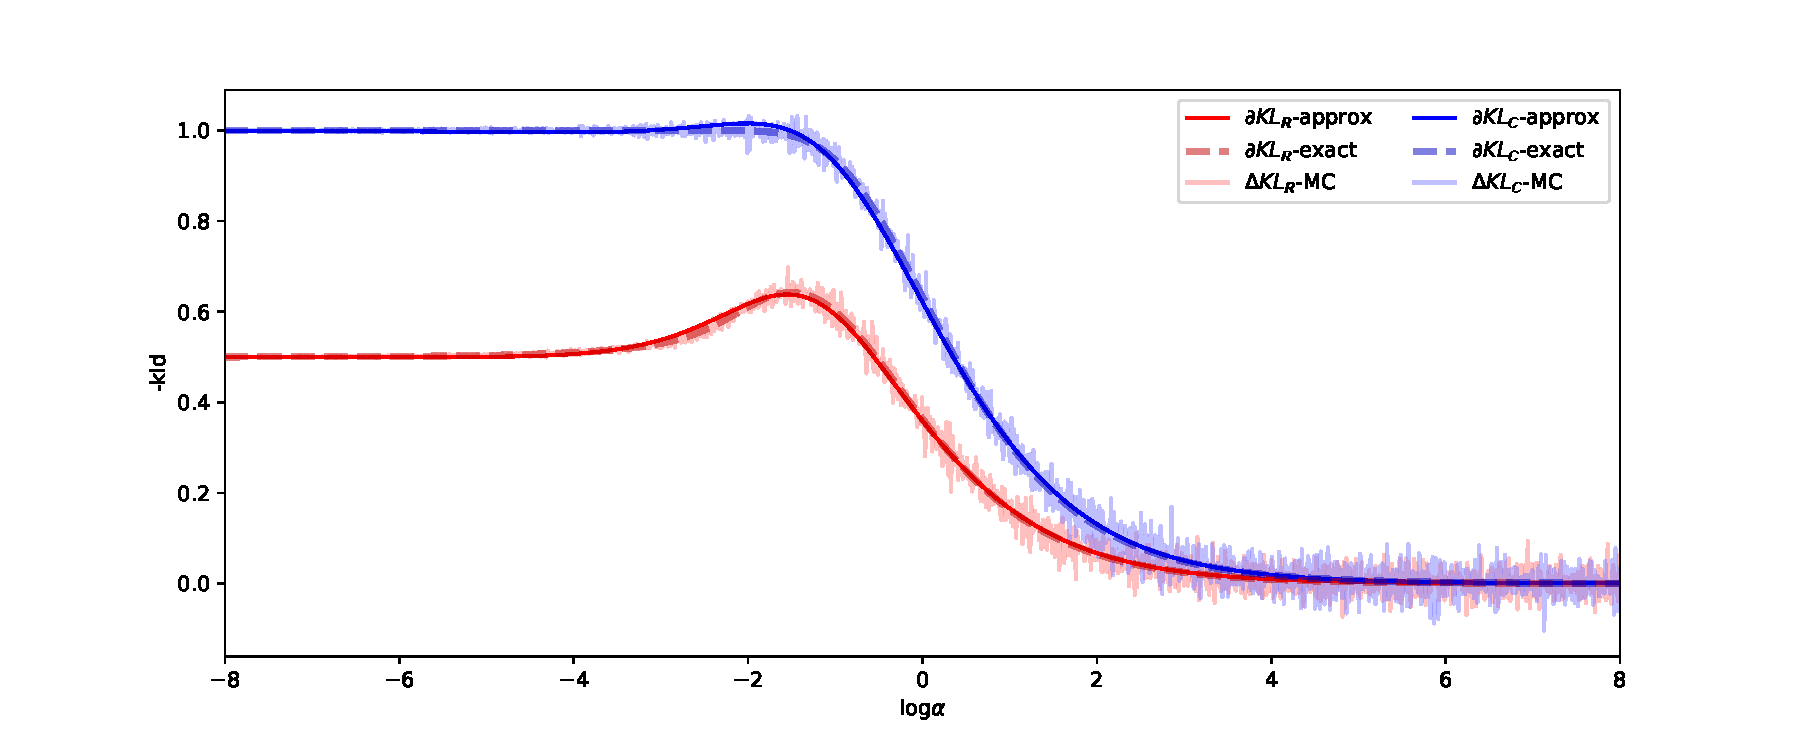
\includegraphics[draft]{../notebooks/assets/grad_log.pdf}
  \end{subfigure}
  \caption{Fit of the regression \cite{molchanov_variational_2017}, and the accuracy of
  the derivative wrt $\log{\alpha}$.}
  \label{fig:molchanov-derivative-replica}
\end{figure}

Now in SGD (and specifically in SGVB) we are concerned more with the gradient field, induced
by the potential (which is the loss function), rather than the value itself. Thus, as far as
the regularizing penalty term is concerned, which is used to regularize the loss objective,
we can essentially ignore it's forward pass value (level) and just compute its gradient
(subgradient, normal cone) with respect the parameter of interest in sgd. (unless it is a
part of a constraint, ie. downstream computation)

% subsection real-chisq-grad (end)

\subsection{Backpropagation through $\cplx$-networks} % (fold)
\label{sub:wirtinger_calculus}

TLDR: we use Wirtinger calculus!

% essential intro into Wirtinger calculus (CR)
Take $f\colon \cplx \to \cplx$ and identify it with $F\colon \real^2 \to \cplx$ function
via $F(u, v) = f(z)\vert_{z=u + j v}$. Wirtinger calculus introduces two formal derivative
operators \rewrite{(this seems to be very verbatim)}
$
  \tfrac{\partial}{\partial z}
    = \tfrac12 \bigl(
      \tfrac{\partial}{\partial u}
      - j \tfrac{\partial}{\partial v}
    \bigr)
$ and $
  \tfrac{\partial}{\partial \conj{z}}
    = \tfrac12 \bigl(
      \tfrac{\partial}{\partial u}
      + j \tfrac{\partial}{\partial v}
    \bigr)
$, defines $dz = du + j dv$, $d\conj{z} = du - j dv$, and the differential of $f$ as
$$
df = \tfrac{\partial f}{\partial z} dz
    + \tfrac{\partial f}{\partial \conj{z}} d\conj{z}
   % = \tfrac12\bigl(
   %    \tfrac{\partial}{\partial u}
   %    - j \tfrac{\partial}{\partial v}
   % \bigr) F (du - j dv)
   % + \tfrac12\bigl(
   %    \tfrac{\partial}{\partial u}
   %    + j \tfrac{\partial}{\partial v}
   % \bigr) F (du - j dv)
   % = \tfrac12 \bigl(
   %    \tfrac{\partial F}{\partial u} du - j \tfrac{\partial F}{\partial v} du
   %    + j \tfrac{\partial F}{\partial u} dv + \tfrac{\partial F}{\partial v} dv
   % \bigr)
   % + \tfrac12 \bigl(
   %    \tfrac{\partial F}{\partial u} du + j \tfrac{\partial F}{\partial v} du
   %    - j \tfrac{\partial F}{\partial u} dv + \tfrac{\partial F}{\partial v} dv
   % \bigr)
   = \tfrac{\partial F}{\partial u} du
     + \tfrac{\partial F}{\partial v} dv
   = dF
  \,. $$
Thus the complex value and its conjugate are treated as independent variables. In this notation
Cauchy-Riemann conditions are expressed as $
  \tfrac{\partial f}{\partial \conj{z}} = 0
$, or $
  -j\tfrac{\partial F}{\partial v} = \tfrac{\partial F}{\partial v}
$. These conditions impose a rigid structure on real and imaginary parts of $F(u, v)$, namely $
  \tfrac{\partial F_{\Re }}{\partial u} = \tfrac{\partial F_{\Im }}{\partial v}
$ and $
  \tfrac{\partial F_{\Re }}{\partial v} = - \tfrac{\partial F_{\Im }}{\partial u}
$. Thus Wirtinger calculus subsumes the usual $\cplx$-calculus, when $
  \tfrac{\partial f}{\partial \conj{z}} = 0
$, i.e. $
  f(z)
    % = g(z, \conj{z})
    = F(\tfrac12 (z + \conj{z}), \tfrac1{j 2} (z - \conj{z}))
$ does not depend on $\conj{z}$.

For a real-valued $f\colon \cplx \to \real$ we have $\conj{f} = f$, whence $
  \tfrac{\partial f}{\partial \conj{z}}
    = \tfrac{\partial \conj{f}}{\partial \conj{z}}
    = \conj{\tfrac{\partial f}{\partial z}}
$. Hence
$$
df
  = \tfrac{\partial f}{\partial z} dz
    + \tfrac{\partial f}{\partial \conj{z}} d\conj{z}
  % = \conj{\tfrac{\partial \conj{f}}{\partial \conj{z}}} dz
  % + \conj{\conj{\tfrac{\partial f}{\partial \conj{z}}} dz}
  = 2 \Re \Bigl(
    \conj{\tfrac{\partial f}{\partial \conj{z}}} dz
  \Bigr)
  = 2 \Re \bigl(
    \tfrac{\partial f}{\partial z} dz
  \bigr)
  \,. $$
Hence the gradient, being the direction of \rewrite{maximal growth} of $f$ at $z$ is given by $
  \tfrac{\partial f}{\partial \conj{z}}
    = \tfrac{\partial F}{\partial u}
      + j \tfrac{\partial F}{\partial v}
$. Thus under Wirtinger calculus it is possible to reuse $\real$-backpropagation.

% Show that $dh(z) = df(g(z)) dg(z)$.
% $h(z) = f(g(z)) = F(G_r(u, v), G_i(u, v)) = H(u, v)$
% $$
% dH
%   = \tfrac{\partial F}{\partial x} \tfrac{\partial G_r}{\partial u} du
%   + \tfrac{\partial F}{\partial x} \tfrac{\partial G_r}{\partial v} dv
%   + \tfrac{\partial F}{\partial y} \tfrac{\partial G_i}{\partial u} du
%   + \tfrac{\partial F}{\partial y} \tfrac{\partial G_i}{\partial v} dv
%   = \tfrac{\partial F}{\partial r} d\Re g(z)
%   + \tfrac{\partial F}{\partial i} d\Im g(z)
%   = df(\Re g(z) + j\Im g(z)) d g(z)
%   = df(g(z)) d g(z)
%   \,. $$

% subsection wirtinger_calculus (end)

\subsection{$\cplx$-Linear operator representation} % (fold)
\label{sub:c-linear_operator_representation}

% proof that such operators exist and are unique (well this is an obvious statement)
Consider $L \colon \cplx^m \to \cplx^n$ -- linear in $\cplx$. Then $
  L(u + jv) = L u + j L v
$ for any $u, v \in \real^m$, which implies that the effect of $L$ as $\cplx$-linear
operator is determined by its restriction onto $\real^n$. Let $
  F = L\vert_{\real^m}
  \colon \real^m \to \cplx^n
$ and observe that $F_r = \Re \circ F$ and $F_i = \Im \circ F$ are $\real$-linear operators
such that $F = F_r + j F_i$ (pointwise). Indeed,
$$
  F_r(a + \lambda b)
  % = \Re F(a + \lambda b)
  = \Re L(a + \lambda b)
  % = \Re \bigl( L a + \lambda L b \bigr)
  = \Re L a + \lambda \Re L b
  % = \Re F a + \lambda \Re F b
  = F_r a + \lambda F_r b
  \,. $$
Therefore for any $\cplx$-linear operator $L$ there are $\real$-linear operators $U, V$
such that
$$
L z 
  = (U + j V) (\Re z + j \Im z)
  % = (U + j V) \Re z + j (U + j V) \Im z
  % = U \Re z + j V \Re z + j \bigl(U \Im z + j V \Im z \bigr)
  = U \Re z - V \Im z + j \bigl( V \Re z + U \Im z \bigr)
  % = (U + j V) z
  \,. $$
Uniqueness of these operators follows, if this decomposition is applied to any $z$ with
$\Im z = 0$.

% subsection c-linear_operator_representation (end)

\subsubsection{MGF of a noncentral $\chi^2$} % (fold)
\label{ssub:mgf_of_a_noncentral_chi}

Consider the mgf of $W$:
$$
M_W(t)
  = \mathbb{E}(e^{Wt})
  = \prod_i \mathbb{E}(e^{(\mu_i + z_i)^2 t})
  \,, $$
by independence. Now for $z \sim \mathcal{N}(\mu, 1)$
$$
\mathbb{E}(e^{z^2 t})
  = \tfrac1{\sqrt{2\pi}}
  \int_{-\infty}^{+\infty}
      e^{z^2 t} e^{-\tfrac{(z-\mu)^2}2}
  dz
  \,. $$
Now, for $t < \tfrac12$
$$
z^2 t - \tfrac{(z - \mu)^2}2
  = - \tfrac12 (1 - 2t) z^2 + z \mu - \tfrac{\mu^2}2
  % = - \tfrac12 (1 - 2t) \bigl(
  %   z^2 - 2 z \tfrac\mu{1 - 2t} + \tfrac{\mu^2}{1 - 2t}
  % \bigr)
  % = - \tfrac12 (1 - 2t) \bigl( z - \tfrac\mu{1 - 2t} \bigr)^2
  % - \tfrac12 (1 - 2t) \bigl(
  %   \tfrac{\mu^2}{1 - 2t}
  %   - \tfrac{\mu^2}{(1 - 2t)^2}
  % \bigr)
  % = - \tfrac12 (1 - 2t) \bigl( z - \tfrac\mu{1 - 2t} \bigr)^2
  %   - \tfrac{\mu^2}2 \bigl(
  %   \tfrac{1 - 2t}{1 - 2t} - \tfrac1{1 - 2t}
  % \bigr)
  % = - \tfrac12 (1 - 2t) \bigl( z - \tfrac\mu{1 - 2t} \bigr)^2
  %   + \tfrac{\mu^2}2 \tfrac{2t}{1 - 2t}
  = - \tfrac12 (1 - 2t) \bigl( z - \tfrac\mu{1 - 2t} \bigr)^2
    + \mu^2 \tfrac{t}{1 - 2t}
  \,, $$
whence
\begin{multline}
  \mathbb{E}(e^{z^2 t})
    = \tfrac1{\sqrt{2\pi}}
      \int_{-\infty}^{+\infty}
        e^{z^2 t} e^{-\tfrac{(z-\mu)^2}2}
      \, dz
    % = e^{\mu^2 \tfrac{t}{1 - 2t}}
    %   \tfrac1{\sqrt{2\pi}}
    %   \int_{-\infty}^{+\infty}
    %     e^{- \tfrac12 (1 - 2t) \bigl( z - \tfrac\mu{1 - 2t} \bigr)^2}
    %   \, dz
    \\= e^{\mu^2 \tfrac{t}{1 - 2t}}
      \tfrac1{\sqrt{2\pi}}
      \int_{-\infty}^{+\infty}
        e^{- \tfrac12 (1 - 2t) z^2}
      \, dz
    % = [u = \sqrt{1 - 2t} z]
    % = e^{\mu^2 \tfrac{t}{1 - 2t}}
    %   \tfrac1{\sqrt{2\pi}}
    %   \int_{-\infty}^{+\infty}
    %     e^{- \tfrac12 u^2}
    %   \, \tfrac{du}{\sqrt{1 - 2t}}
    = \tfrac{
        \exp{\{\mu^2 \tfrac{t}{1 - 2t}\}}
    }{\sqrt{1 - 2t}}
    \,.
\end{multline}
Therefore
$$
M_W(t)
  = \mathbb{E}(e^{Wt})
  = \prod_i \tfrac{
      e^{\mu_i^2 \tfrac{t}{1 - 2t}}
    }{\sqrt{1 - 2t}}
  % = e^{\lambda \tfrac{t}{1 - 2t}}
  %   (1 - 2t)^{-\tfrac{m}2}
  % = e^{\lambda \tfrac{- t}{2t - 1}}
  %   (1 - 2t)^{-\tfrac{m}2}
  % = e^{\tfrac\lambda2 \tfrac{1 - 2t - 1}{2t - 1}}
  %   (1 - 2t)^{-\tfrac{m}2}
  % = e^{- \tfrac\lambda2 (1 + \tfrac1{2t - 1})}
  %   (1 - 2t)^{-\tfrac{m}2} 
  = e^{- \tfrac\lambda2} e^{\tfrac\lambda2 \tfrac1{1 - 2t}}
  (1 - 2t)^{-\tfrac{m}2}
  \,. $$
Expanding the exponential as infinite series:
\begin{multline}
  M_W(t)
    = e^{- \tfrac\lambda2} e^{\tfrac\lambda2 \tfrac1{1 - 2t}}
    (1 - 2t)^{-\tfrac{m}2}
    % = e^{- \tfrac\lambda2} (1 - 2t)^{-\tfrac{m}2}
    %   \sum_{n \geq 0} \tfrac{\bigl(\tfrac\lambda2\bigr)^n}{n! (1 - 2t)^n}
    \\= \sum_{n \geq 0} \tfrac{e^{- \tfrac\lambda2} \bigl(\tfrac\lambda2\bigr)^n}{n!}
        (1 - 2t)^{-\tfrac{2n + m}2}
    = \sum_{n \geq 0} \tfrac{e^{- \tfrac\lambda2} \bigl(\tfrac\lambda2\bigr)^n}{n!}
        \mathbb{E}_{x \sim \chi^2_{m + 2n}}(e^{x t})
    \,.
\end{multline}

% subsubsection mgf_of_a_noncentral_chi (end)

% section appendix (end)

%%%%%%%%%%%%%%%%%%%%%%%%%%%%%%%%%%%%%%%%%%%%%%%%%%%%%%%%%%%%%%%%%%%%%%%%%%%%%%%%%%%%%%%%%%%%%%%%%%%

\clearpage


\section{Trunk} % (fold)
\label{sec:trunk}

In the case of $\real$-valued variational dropout \cite{kingma_variational_2015} approximate
\eqref{eq:expect-improper-term-cplx} by a non-linear regression, fit to the Monte-Carlo estimates
of the expectation for $\alpha$ varying over a logarithmic grid. This approximation was greatly
refined in \cite{molchanov_variational_2017} -- an improvement that enabled doing away with
the clipping of the dropout rate (relevance score) $\alpha$. In fact in the real case the analogue
of the last term in \eqref{eq:expect-improper-term-cplx} is half the log-moment of a non-central
$\chi^2$ distribution with shape $1$ and non-centrality $\lambda = \tfrac1{\alpha}$. Unfortunately,
there is no known expression (even involving special functions) for this expectation for
$\chi^2_m$ with odd shape parameter $m$ (degrees of freedom) \verify{this}. Quite fortunately
there is one for even degrees of freedom.

%%%%%%%
\todo{why this is better than a general $\cplx$-gaussian? Three parameters?}

\important{``pytorch'' specific}
Otherwise we have to offload the values from the device to cpu, compute the special
function there, and transfer back.

Why sparsity matters, why $\cplx$ networks?

Where are $\cplx$-networks used? and do these applications warrant sparsity?

Gist of the LRP (kingmaetal2015)
translating uncertainty (randomness) from parameters to activations
  adds noise -- helps regularization
  emulates one draw per batch element -- decorrelates gradient within the batch
  reduces computations (memory), leverages batched matmuls (or convos)
  decreases variance of the gradient

additive noise reparameterization (molchanov\_variational\_2017) $(\mu, \alpha \mu^2)$:
  less noisy gradient wrt $\mu$, $\alpha$ recomputed on-the-fly

\subsection{$\cplx$-valued networks} % (fold)
\label{sub:c_valued_networks}

In this section i remind the reader what the complex-valued networks are, how
they are implemented and how much of $\cplx$-ness they have. Mention careful
design.

I will describe the linear layers (dense, masked, and convolutions) and
activations borrowed straight from the $\real$-values networks. Then i shall
mention that this has been tried before and list papers that one way or another
address $\cplx$-data processing with neural networks.


It is worth pointing out that the key advantage of
the $\cplx$-constraints is that they permit use of Strassen's $3$M multiplication algorithm,
potentially \verify{saving up} to $25\%$ on floating point multiplications. \todo{
  in contrast to what? to na{\:i}ve (obvious)? to paired-$\real$ ($2 \times 2$-$2\times 1$
  -- 4 fmul)?
}

% subsection c_valued_networks (end)

\section{Complex Variational Dropout} % (fold)
\label{sec:complex_variational_dropout}

In this section we outline and derive the variational dropout technique for complex-%
valued networks, which re-traces the evolution of dropout technique for real-valued
weights.



% a second take on bayesian inference
The core question of Bayesian analysis is concerned with the distribution of the data model
after observing data and given the initial belief about it. The data model is typically a joint
distribution on the sample, which includes assumptions regarding independence and (conditional)
factorization of the distribution of each individual data point. In our case we suppose that
the data $
  \mathcal{D} = (z_i)_{i=1}^m
$, $z_i = (x_i, y_i)$ is independent and identically distributed under our model $m$: $
  p(\mathcal{D}\mid m)
    = \prod_i p(z_i\mid m)
$. The models we  our model $m$ comes from a parametric conditional distribution family, e.g. $
  p(z \mid m)
    = p(y \mid x, m) p(x \mid m)
    = p(y \mid x, m) p(x)
$ and $
  p(y \mid x, m)
    = \mathcal{N}\bigl(
      y\,\mid\, \mu_\omega(x)\,, \sigma^2_\omega(x)
    \bigr)
$, then we can (and do) identify $m$ with its parameters $\omega$. Instead of iid data in
$\mathcal{D}$, we could have assumed a Gaussian Process data model $
  y(x) \sim \mathrm{GP}(\mu, K)
$ for the mean function and covariance kernel $
  \mu
    \colon \mathcal{X} \to \real^d
$ and $
  K \colon \mathcal{X} \times \mathcal{X}
    \to \real^{d\times d}
$.

In the framework of Bayesian Inference we use the Bayes's rule as an exact method for deriving
the posterior parameter distribution from the likelihood of the data model and model's prior:
$
  p(\omega \mid \mathcal{D})
    = \tfrac{
      p(\mathcal{D} \mid \omega) \pi(\omega)
    }{
      p(\mathcal{D})
    }
$. Typically, exact inference involves an analytically intractable integrals, e.g. in the
denominator of the posterior $
  p(\mathcal{D})
    = \int p(\mathcal{D} \mid \omega) \pi(\omega) d\omega
$, or derived distributions, such as the predictive distribution $
  p(y \mid x, \mathcal{D})
    = \int p(y \mid x, \omega) p(\omega \mid \mathcal{D}) d\omega
$.

Variational Inference recasts the problem of posterior derivation into functional optimization
framework. The main idea is to find the closest approximation to the posterior $
  p(\omega \mid \mathcal{D})
$ in some family $
  \mathcal{Q}
$ of approximating distributions $
  q(\omega)
$ on the parameters $\omega$ of the model $m$ (or the model itself). The proximity between
distributions is measured either using MMD metric via embedding into some universal RKHS,
\cite{citation_needed}, Wasserstein \cite{citation_needed} \cite{citation_needed}, total
variation norm \cite{citation_needed}, or $f$-divergences
% $
%   \mathbb{E}_{\omega \sim q(\omega)} f\bigl(
%       \tfrac{p(\omega)}{q(\omega)}
%     \bigr)
% $ for a convex $f$ with $f(1) = 0$
\cite{citation_needed}, specifically Kullback-Leibler divergence. The key trade off in Variational
Inference is the choice of the approximating family that is rich enough to get close to the true
posterior, yet simple enough to sample from or for inferring derived distributions via Bayesian
averaging.

Despite the effort to simplify the bayesian analysis in the most commonly encountered cases
variational inference still requires dealing with analytically intractable expectations,
\cite{citation_needed}. This issue is dealt with by giving up deterministic precision to
gain efficiency from stochastic, since inaccuracies and assumptions are inevitable, especially
when modelling observations.

% a verbatim setion from my mlss2019 bdl notebook
In Bayesian Inference (\textbf{BI}) we \textit{assume} that the observation data $D$ follows a
\textit{model} $m$ with data generating distribution $p(D \mid m, \omega)$ \textit{governed by
unknown parameters} $\omega$. The goal of \textbf{BI} is to reason about the model and/or its
parameters, and new data given the observed data $D$ and our assumptions, i.e to seek the
\textbf{posterior} parameter and predictive distributions:

\begin{align}
p(d \mid D, m)
  &
  % = \mathbb{E}_{
  %   \omega \sim p(\omega \mid D, m)
  % } p(d \mid D, \omega, m)
  = \int p(d \mid D, \omega, m) p(\omega \mid D, m) d\omega
  \,, \\
p(\omega \mid D, m)
  &
  = \frac{p(D \mid \omega, m) \, \pi(\omega \mid m)}{p(D \mid m)}
  \,,
\end{align}
where
\begin{itemize}
  \item the \textbf{prior} distribution $\pi(\omega \mid m)$ reflects our belief before
  having made the observations
  \item the data distribution $p(D \mid \omega, m)$ reflects our assumptions about the data
  generating process, and determines the model \textbf{likelihood} (Gaussian, Categorical,
  Poisson etc.)
\end{itemize}
Unless the distributions and likelihoods are conjugate, posterior in Bayesian inference is
typically intractable and it is common to resort to \textbf{Variational Inference} or
\textbf{Monte Carlo} approximations.

Since inference using the exact posterior is rarely tractable, efficient and unbiased approximation
schemes are typically used. One such scheme is Variational Inference, which casts the inference
task into the domain of optimization problems over some appropriately chosen the posterior
distribution approximation family. The key idea of the former is to seek an approximation
$q(\omega)$ to the intractable posterior $p(\omega \mid D, m)$, via a variational optimization
problem over some parametric family of distributions $\mathcal{Q}$:
$$
q^*(\omega)
    \in \arg \min_{q\in \mathcal{Q}}
      \mathrm{KL}(q(\omega) \| p(\omega \mid D, m))
  \,, $$
where the Kullback-Leibler divergence between $P$ and $Q$ ($P\ll Q$) with densities $p$ and $q$,
respectively, is given by
$$
\mathrm{KL}(q(\omega) \| p(\omega))
  % = \mathbb{E}_{\omega \sim Q} \log \tfrac{dQ}{dP}(\omega)
  = \mathbb{E}_{\omega \sim q(\omega)}
    \log \tfrac{q(\omega)}{p(\omega)}
  \,.
  % \tag{kl-div}
  $$

Note that the family of variational approximations $\mathcal{Q}$ can be structured
\textbf{arbitrarily}: point-mass, products, mixture, dependent on input, having mixed hierarchical
structure, -- any distribution, even unnormalized. Although computing the divergence w.r.t.
the unknown posterior is still hard and intractable, it is possible to do away with it
through the following identity, which is based on the Bayes rule.

For \textbf{any} $q(\omega) \ll p(\omega \mid D; \phi)$ and any model $m$

\begin{align}
\overbrace{
  \log p(D \mid m)
}^{\text{evidence}}
  &= \overbrace{
    \mathbb{E}_{\omega \sim q} \log p(D\mid \omega, m)
  }^{\text{expected conditional likelihood}}
  - \overbrace{
    \mathrm{KL}(q(\omega)\| \pi(\omega \mid m))
  }^{\text{proximity to prior belief}}
  \\
  &+ \underbrace{
    \mathrm{KL}(q(\omega)\| p(\omega \mid D, m))
  }_{\text{posterior approximation}}
\,.
\tag{master-identity}
\end{align}
Instead of minimizing the divergence of the approximation from the posterior, we can maximize
the \textbf{Evidence Lower Bound} with respect to $q(\omega)$:
$$
q^* \in
  \arg\max_{q\in Q}
    \mathcal{L}(q)
    = \mathbb{E}_{\omega \sim q} \log p(D\mid \omega, m)
      - \mathrm{KL}(q(\omega)\| \pi(\omega \mid m))
  \,.
  % \tag{max-ELBO}
  $$
The intuition is that the expected $\log$-likelihood favours $q$ that place their mass on
parameters $\omega$ that explain $D$ under the specified model $m$. At the same time
the negative KL-divergence discourages the approximation $q$ from straying too far away
from to the prior belief $\pi$ under $m$.

We usually consider the following setup (conditioning on model $m$ is omitted):
\begin{itemize}
  \item the likelihood factorizes $
    p(D \mid \omega)
        = \prod_i p(y_i, x_i \mid \omega)
        \propto \prod_i p(y_i \mid x_i, \omega)
  $
  for $D = (x_i, y_i)_{i=1}^N$

  \item the variational posterior approximation is parameterized by $\theta$: $q(\omega \mid \theta)$

  \item the prior on $\omega$ also depends on hyper-parameters $\lambda$, that can be fixed,
  or variable ($\pi(\omega \mid \lambda)$).
\end{itemize}

In this case the variational objective (evidence lower bound)
$$
\log p(D\mid \lambda )
  \geq \mathcal{L}(\theta, \lambda)
    = \mathbb{E}_{\omega \sim q(\omega \mid \theta)}
      \sum_i \log p_\phi(y_i \mid x_i, \omega)
    - KL(q(\omega \mid \theta) \| \pi(\omega \mid \lambda))
  \,, $$
is maximized with respect to $\theta$ (to approximate the posterior).

Priors can be
\begin{itemize}
  \item \textit{subjective}, i.e. reflecting prior beliefs (but not arbitrary)
  \item \textit{objective}, i.e. reflecting our lack of knowledge
  \item \title{empirical}, i.e. learnt from the observed data (optimized over
  hyper-parameters $\lambda$)
\end{itemize}

The stochastic variant of ELBO is formed by randomly batching
the dataset $D$:
$$
\mathcal{L}(\theta, \lambda)
  \approx \mathcal{L}_\mathrm{SGVB}(\theta, \lambda)
  = \lvert D \rvert \biggl(
    \tfrac1{\lvert B \rvert}
      \sum_{b \in B} \mathbb{E}_{\omega \sim q(\omega \mid \theta)}
        \log p(y_b \mid x_b, \omega)
  \biggr)
  - KL(q(\omega \mid \theta) \| \pi(\omega \mid \lambda))
  \,. $$

Stochastic optimization follows noisy unbiased gradient estimates, which are usually cheap and
allow escaping from local optima, but optimize the objective in expectation. In order to get
a gradient of $
  F_\theta = \mathbb{E}_{\omega \sim q(\omega \mid \theta)} f(\omega)
$ w.r.t $\theta$ we use either:
\begin{itemize}
  \item (REINFORCE) $
    \nabla_\theta F_\theta
      = \mathbb{E}_{\omega \sim q(\omega \mid \theta)}
        (f(\omega) - b_\theta) \nabla_\theta \log q(\omega \mid \theta)
  $ for some $b_\theta$ that is used to control variance

  \item (reparameterization) $
    \nabla_\theta F_\theta
      = \nabla_\theta \mathbb{E}_{\varepsilon \sim q(\varepsilon)}
        f(g(\theta; \varepsilon))
      = \mathbb{E}_{\varepsilon \sim q(\varepsilon)}
        \nabla_\theta g(\theta; \varepsilon)
          \nabla_\omega f(\omega) \big\vert_{\omega = g(\theta; \varepsilon)}
    $ when there are $q$ and differentiable $g$, such that sampling from $
      q(\omega \mid \theta)
    $ is equivalent to $
      \omega = g(\theta; \varepsilon)
    $ with $\varepsilon \sim q(\varepsilon)$
\end{itemize}

The variational approximation might yield high dimensional integrals, which are slow/prohibitive
to compute. To make the computations faster without foregoing much of the precision, we may use
Monte Carlo estimator:
$$
\mathbb{E}_{\omega \sim q(\omega\mid \theta)} \, f(\omega)
  \overset{\text{MC}}{\approx}
    \frac1{\lvert \mathcal{W}\rvert}
      \sum_{\omega \in \mathcal{W}} f(\omega)
  \,, $$
where $\mathcal{W} = (\omega_b)_{b=1}^B$ is a sample of independent draws from $
  q(\omega\mid \theta)
$. If we also approximate the expectation wrt model parameters in the gradient of ELBO via Monte
Carlo we get the \textbf{doubly stochastic variational objective}:
$$
\nabla_\theta \mathcal{L}_\mathrm{DSVB}(\theta, \lambda)
  \approx
    \lvert D \rvert \biggl(
      \tfrac1{\lvert B \rvert}
        \sum_{b \in B}
          \mathop{gradient}(x_b, y_b)
    \biggr)
    - \nabla_\theta KL(q(\omega \mid \theta) \| \pi(\omega \mid \lambda))
  \,, $$
where `gradient` is $
  \nabla_\theta
    \mathbb{E}_{\omega \sim q(\omega \mid \theta)}
      \log p(y \mid x, \omega)
$ using one of the approaches above, typically approximated using one independent draw of $\omega$
per $b\in B$. We can use a similar sampling approach to compute the gradient of the divergence term.

We can estimate the divergence term in the ELBO with Monte Carlo, or, for example, for the
predictive distribution we have
\begin{align}
\mathbb{E}_{y\sim p(y\mid x, D, m)} \, g(y)
  &
  \overset{\text{BI}}{=}
    \mathbb{E}_{\omega\sim p(\omega \mid D, m)}
      \mathbb{E}_{y\sim p(y\mid x, \omega, D, m)} \, g(y)
  \\
  &
  \overset{\text{VI}}{\approx}
    \mathbb{E}_{\omega\sim q(\omega)}
      \mathbb{E}_{y\sim p(y\mid x, \omega, D, m)} \, g(y)
  \\
  &
  \overset{\text{MC}}{\approx}
    % \hat{\mathbb{E}}_{\omega \sim \mathcal{W}}
    %   \mathbb{E}_{y\sim p(y\mid x, \omega, D, m)} \, g(y)
    \frac1{\lvert \mathcal{W}\rvert} \sum_{\omega \in \mathcal{W}}
      \mathbb{E}_{y\sim p(y\mid x, \omega, D, m)} \, g(y)
  \,,
\end{align}
where $\mathcal{W} = (\omega_b)_{b=1}^B \sim q(\omega)$ -- iid samples from the variational
approximation.

\bigskip

% on bernoulli dropout
Bernoulli dropout alleviates the problem of overfitting

% on gaussian dropout

% revirew of kingma and lrt
The key contributions of \cite{kingma_variational_2015} are reinterpretation of dropout
as a variational inference method and the analysis of the effects that the local reparameterization
trick has on the efficiency of the gradient estimator in stochastic variational inference,
\cite{citation_needed}.

\cite{kingmaetal2015} argue that Gaussian dropout, being a multiplicative parameter noise,
can be interpreted as variational inference via factorized Gaussian posterior approximation
$q(\omega)$ that optimizes the $\log$-likelihood term from the Evidence Lower Bound. In a fully
Bayesian treatment, the dropout rate $p \in (0, 1)$, which governs the regularization strength,
would appear in the KL-divergence term of ELBO through the corresponding odds $
  \alpha = \tfrac{p}{1-p}
$, which acts a variance scaling factor in the posterior approximation. Having made $\alpha$
a learnable parameter of the variational approximation, \cite{kingmaetal2015} natuallry propose
letting it vary on the per-parameter basis, which allows for even more flexible posterior
approximations. % who proposed sparsification?

The local reparameterization trick, proposed by \cite{citation_wang_menning_2013} in the context
of Bernoulli and Gaussian dropout regularization techniques \cite{citation_needed}, translates
the uncertainty about global parameters to noise in the local intermediate state and utilizes
the closure of Gaussian distribution under affine transformations. Computational advantage of
the trick is that activation noise is cheaper to sample and store for the purposes of backpropagation,
than independently sampling parameters from the posterior approximation individually for each
element of the minibatch. As far as Bayesian inference is concerned, \cite{kingma_variational_2015}
have shown that trick's beneficial effects on minibatch SGD convergence come via two mechanisms
of likelihood gradient estimator's efficiency: decorrelation within the batch (independent noise
draws) and variance reduction through local transfer of parameter uncertainty to activation noise.

\begin{quote}

in practice the performance of stochastic gradient methods depends on the variance of the gradient
field

sampling the activations directly, without the parameter randomness gives a low cost efficient
MC estimator (statistical efficiency).

the gradient in sgvb is unbiased estimate of the $\log$-likelihood part of the elbo

\end{quote}


% a comment on Bernoulli dropout
The key idea of Bernoulli dropout is to randomly mask input features of a layer during
training with in order to learn decorrelated feature maps. In a recent study of network
capacity for multitask learning, \cite{multitask2019}, it was shown, that associating
each dataset (task) with a context, that masks a subset of the parameters, allows non-%
destructive `packing' of the tasks in orthogonal on average `subsets' of a single set
of weights, without much interference between tasks. This lends support for beneficial
effects of Bernulli Dropout on test performance, since, in effect, the network learns
to perform well on identical copies of the same task with different (binary) contexts
with a single parameter set.

% exposition

% plan

A linear layer is parameterized by $W \in\real^{n \times m}$ and bias $b\in \real^n$ and
acts on its input $x\in \real^m$ via $y = W x + b$ with $y\in \real^n$. The key idea of
Bernoulli dropout is to mask elements in the matrix $W$ of the layer
with some given probability $p$: $W = \theta \odot \xi$ with $\theta$ being the learnt
weight matrix, and $
  \xi \sim \mathcal{B}(\{0, \tfrac1{1-p}\}, 1-p)
$ -- an iid Bernoulli mask. During training, a dropout mask $\xi$ is used to compute $W$,
and during evaluation the weights are fixed to the expectation of $W$ which is $\theta$.
The discussion and analysis in \cite{kingma_variational_2015}, suggest that drawing one
common dropout mask for all data in the minibatch reduces statistical efficiency the estimator
of the weights' gradient in the stochastic approximation of the evidence lower bound. 

Gaussian dropout works in a similar fashion, except the dropout mask $\xi$ is iid $
  \mathcal{N}(1, \alpha=\tfrac{p}{1-p})
$, i.e. a multiplicative Gaussian noise is injected into the network.

The key idea of Variational Dropout is to assume a Gaussian Mean field variational
approximation of the posterior distribution of linear layer's weights (or convolutional
kernels, with a caveat\footnote).  \footnotetext{
  at each spatial patch of input data the kernel is independently redrawn form the
  VI distribution. This again helps with gradient variance reduction.
}
Weight $W$ are assumed to have independently distributed elements with $
  w_{ij} \sim \mathcal{N}(\theta_{ij}, \sigma^2_{ij})
$.

In fact multiplicative Gaussian dropout on weights $W$ is in fact itself a variational
approximation with variance $\sigma^2_{ij} = \theta_{ij}^2 \tfrac{p}{1-p}$ determined
by the dropout rate.

% set by step we retell the story of kingmaetal2015

Gaussian variational approximation enabled \cite{kingma_variational_2015} propose a
\textit{local reparameterization trick}, which reduces the variance of the gradients
in SGVB and does not resample $W$ per element of a minibatch. It relies the closure
of Gaussian distribution under linear transformations. Indeed, if $W$ is a Gaussian
matrix with independently distributed $
  W_{ij} \sim \mathcal{N}(\theta_{ij}, \sigma^2_{ij})
$, then we have \important{moved}.



and instead
translating the uncertainty from the weights into local output noise of each linear layer.
Without this it would have been necessary to draw new set of random weights per each element
in a mini-batch.

$$
  \mathcal{N}(\theta_{ij}, \alpha \theta^2_{ij})
  \overset{\mathcal{D}}{\sim}
  \theta_{ij} \mathcal{N}(1, \alpha)
  \,, $$

\cite{molchanov_variational_2017} propose additional step in the local reparametrization,
which further reduces the variance of the gradient estimator for each dropped out
weight. Their simple formal change of variables $(\theta, \alpha) \to (\theta, \sigma^2)$
decouples the stochastic component from the weights \rewrite:
$$
  w_{ij} = \theta_{ij} + \theta_{ij} \sqrt{\alpha} \varepsilon_{ij}
  \,\to\,
  w_{ij} = \theta_{ij} + \sigma^2_{ij} \varepsilon_{ij}
  \,, $$
with the appropriate change of variables in the Kullback-Leibler divergence.
($\alpha_{ij} = \tfrac{\sigma_{ij}^2}{\lvert \theta_{ij}\rvert^2}$).

Criticism of \cite{gale_state_2019} implies that $\ell_0$-variational dropout,
proposed by \cite{louizos_learning_2017} and based on the concrete binary distribution
of \cite{maddison_concrete_2016}, works consistently better than the variational
Gaussian dropout.

Maths and related results \cite{pav_moments_2015,taubock_complex-valued_2012},
and \cite{karseras_caution:_2014}

% section complex_variational_dropout (end)

\end{document}